\documentclass[compress]{beamer}
\mode<presentation>
\usetheme{Warsaw}
\usecolortheme{seagull}

%\useoutertheme[subsection=false]{smoothbars}

%\usepackage{stackengine}
%\setbeamertemplate{caption}{\raggedright\insertcaption\par}
\setbeamertemplate{caption}{\insertcaption} 
%\usepackage{caption}
%\usepackage{pgffor}

\usepackage{fancybox}
\usepackage{minibox}

%\usepackage{tcolorbox}
\usepackage{empheq}


%% ====================================== graphics

\usepackage{pgfplots}
\pgfplotsset{width=10cm,compat=1.9}
%\usepgfplotslibrary{external}
%\tikzexternalize
 \usepackage{pgfplotstable}

%\definecolor{markercolor}{RGB}{.49, 1, .63}
\definecolor{markercolor}{RGB}{124.9, 255, 160.65}

\pgfplotsset{
tick label style={font=\scriptsize},
label style={font=\scriptsize},
legend style={font=\scriptsize},
title style={font=\footnotesize}
}

%% ===========================================
\usepackage{stmaryrd}

\usepackage{amsmath,amsfonts,amsthm}

% for FD grid tikz
\usepackage{tikz,amssymb}
\usetikzlibrary{calc}
\newcommand\bound{10}

\usepackage{slopetri}

\useoutertheme{infolines}
\useinnertheme{rectangles}
\usepackage{hhline}
\setbeamercovered{dynamic}

\usepackage{soul}

\usepackage{array}
\usepackage{mathrsfs}
\usepackage[utf8]{inputenc}
\usepackage{listings}
\usepackage{mathtools}
\usepackage{bm}
\usepackage{cancel}


\usepackage{graphicx}
\usepackage{subfig}
\makeatletter
\let\@@magyar@captionfix\relax
\makeatother

\usepackage{color}

\usepackage{bibentry}
\nobibliography*

\theoremstyle{plain}

% vertical bars
\newcommand*{\vertbar}{\rule[-1ex]{0.5pt}{2.5ex}}

\renewcommand{\hat}{\widehat}
\renewcommand{\tilde}{\widetilde}

%% d in integrand
\newcommand*\diff[1]{\mathop{}\!{\mathrm{d}#1}}
\newcommand{\diag}[1]{{\rm diag}\LRp{#1}}
\newcommand{\td}[2]{\frac{{\rm d}#1}{{\rm d}{\rm #2}}}
\newcommand{\pd}[2]{\frac{\partial#1}{\partial#2}}
\newcommand{\nor}[1]{\left\| #1 \right\|}
\newcommand{\LRp}[1]{\left( #1 \right)}
\newcommand{\LRs}[1]{\left[ #1 \right]}
\newcommand{\LRa}[1]{\left\langle #1 \right\rangle}
\newcommand{\LRb}[1]{\left| #1 \right|}
\newcommand{\LRc}[1]{\left\{ #1 \right\}}
\newcommand{\LRceil}[1]{\left\lceil #1 \right\rceil}
\newcommand{\LRu}[1]{\left. #1 \right|}
\newcommand{\pdn}[3]{\frac{\partial^{#3}#1}{\partial#2^{#3}}}
\newcommand{\Grad} {\ensuremath{\nabla}}
\newcommand{\jump}[1] {\ensuremath{\llbracket#1\rrbracket}}
\newcommand{\avg}[1] {\ensuremath{\LRc{\!\{#1\}\!}}}

\graphicspath{{./figs/}}

\renewcommand{\note}[1]{\textcolor{red}{{#1}}}
%\renewcommand{\note}[1]{{\color{blue}{#1}}}


% removes nav symbols
\beamertemplatenavigationsymbolsempty
%\setbeamertemplate{caption}{\raggedright\insertcaption\par}

% defines newblock as null, giving compile issues otherwise
\let\newblock\relax 


\title[Entropy stable ROMs]{	
Entropy stable reduced order modeling of nonlinear conservation laws}
\date[7/17/19]{ICIAM 2019, Valencia, Spain\\ \note{Reduced-order modeling} and data-driven estimation in waves and \note{fluids} \\July 17, 2019}
\author[J.\ Chan]{Jesse Chan}
\institute[Rice CAAM]{\inst{1}Department of Computational and Applied Mathematics}

\begin{document}
\makeatletter
\@addtoreset{subfigure}{framenumber}% subfigure counter resets every frame
\makeatother

\begin{frame}
\maketitle
\end{frame}

%% =================================================

%\frame{
%\frametitle{Discretely entropy stable schemes}
%
%Goal: address the stability and robustness of high order methods for nonlinear conservation laws.
%\begin{columns}
%\begin{column}{.5\textwidth}
%\begin{figure}
%%\vspace{-1em}
%\centering
%%\only<1>{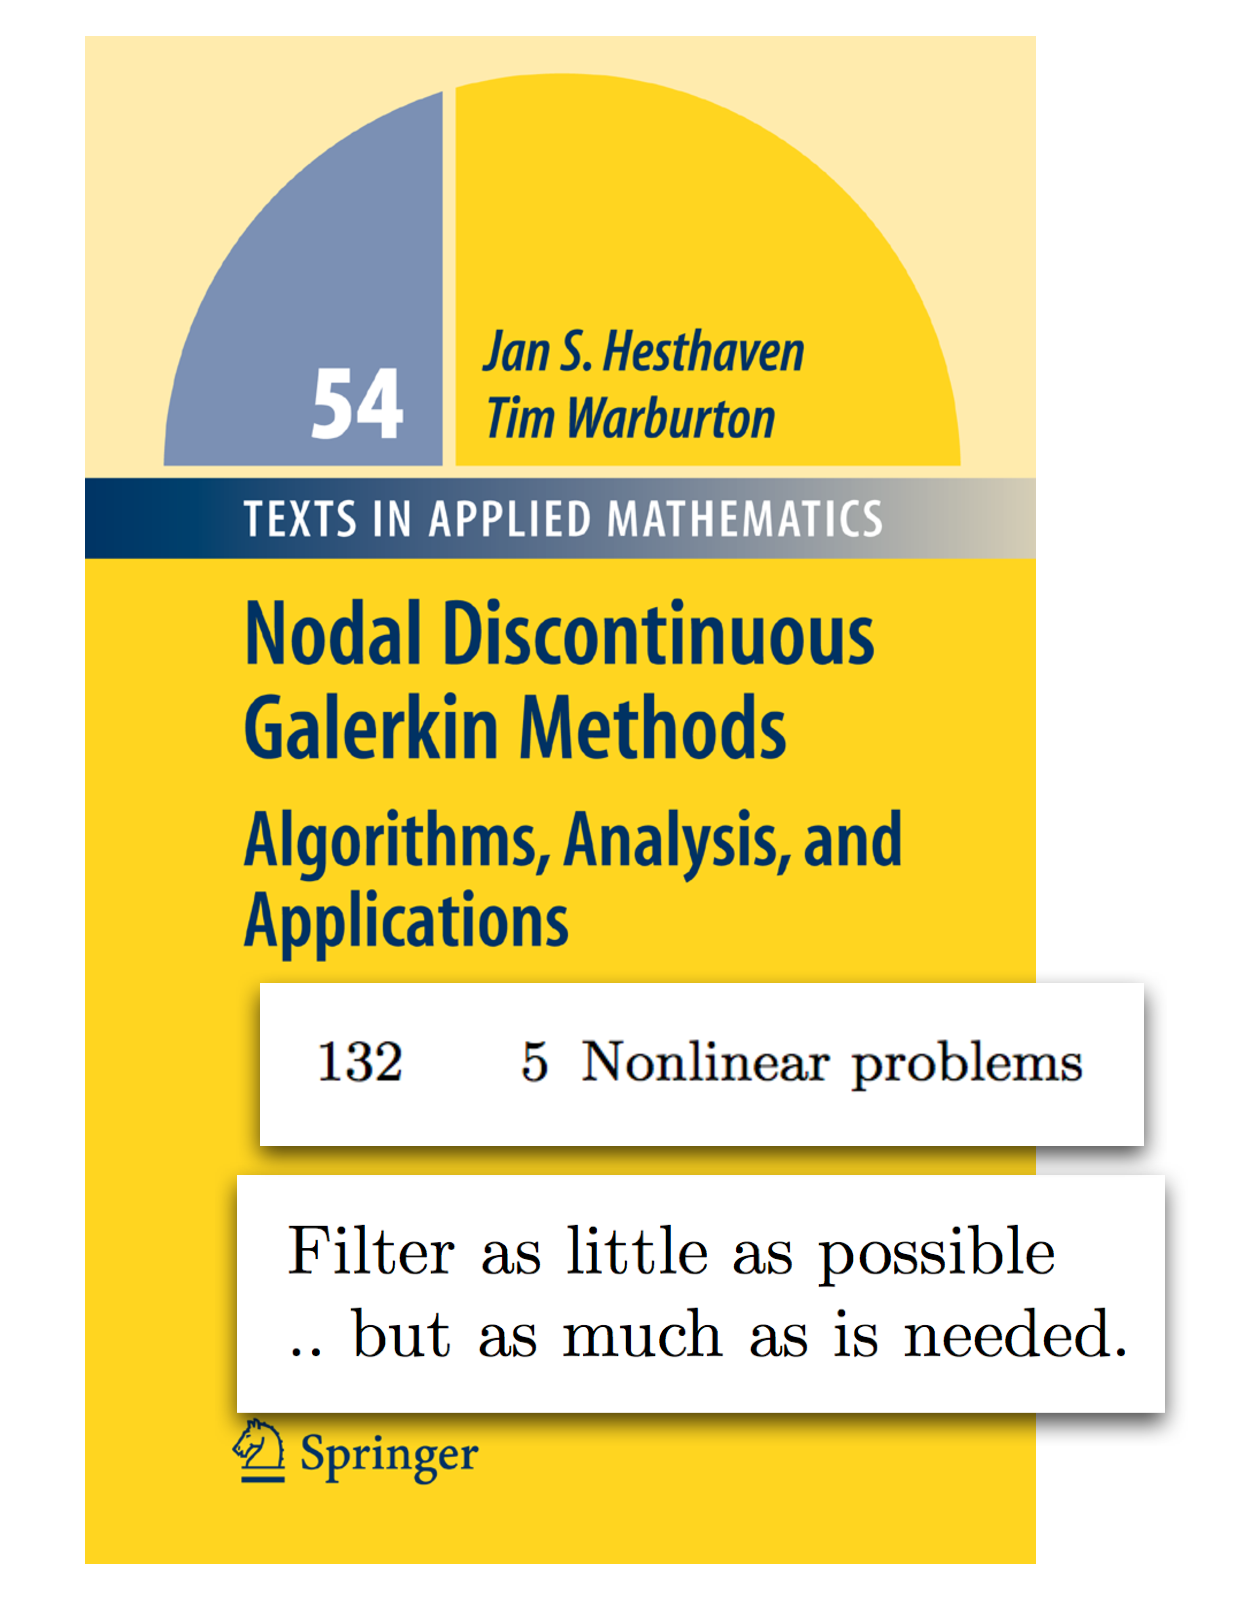
\includegraphics[width=.95\textwidth]{figs/ndgFilter.pdf}}
%%\only<2>{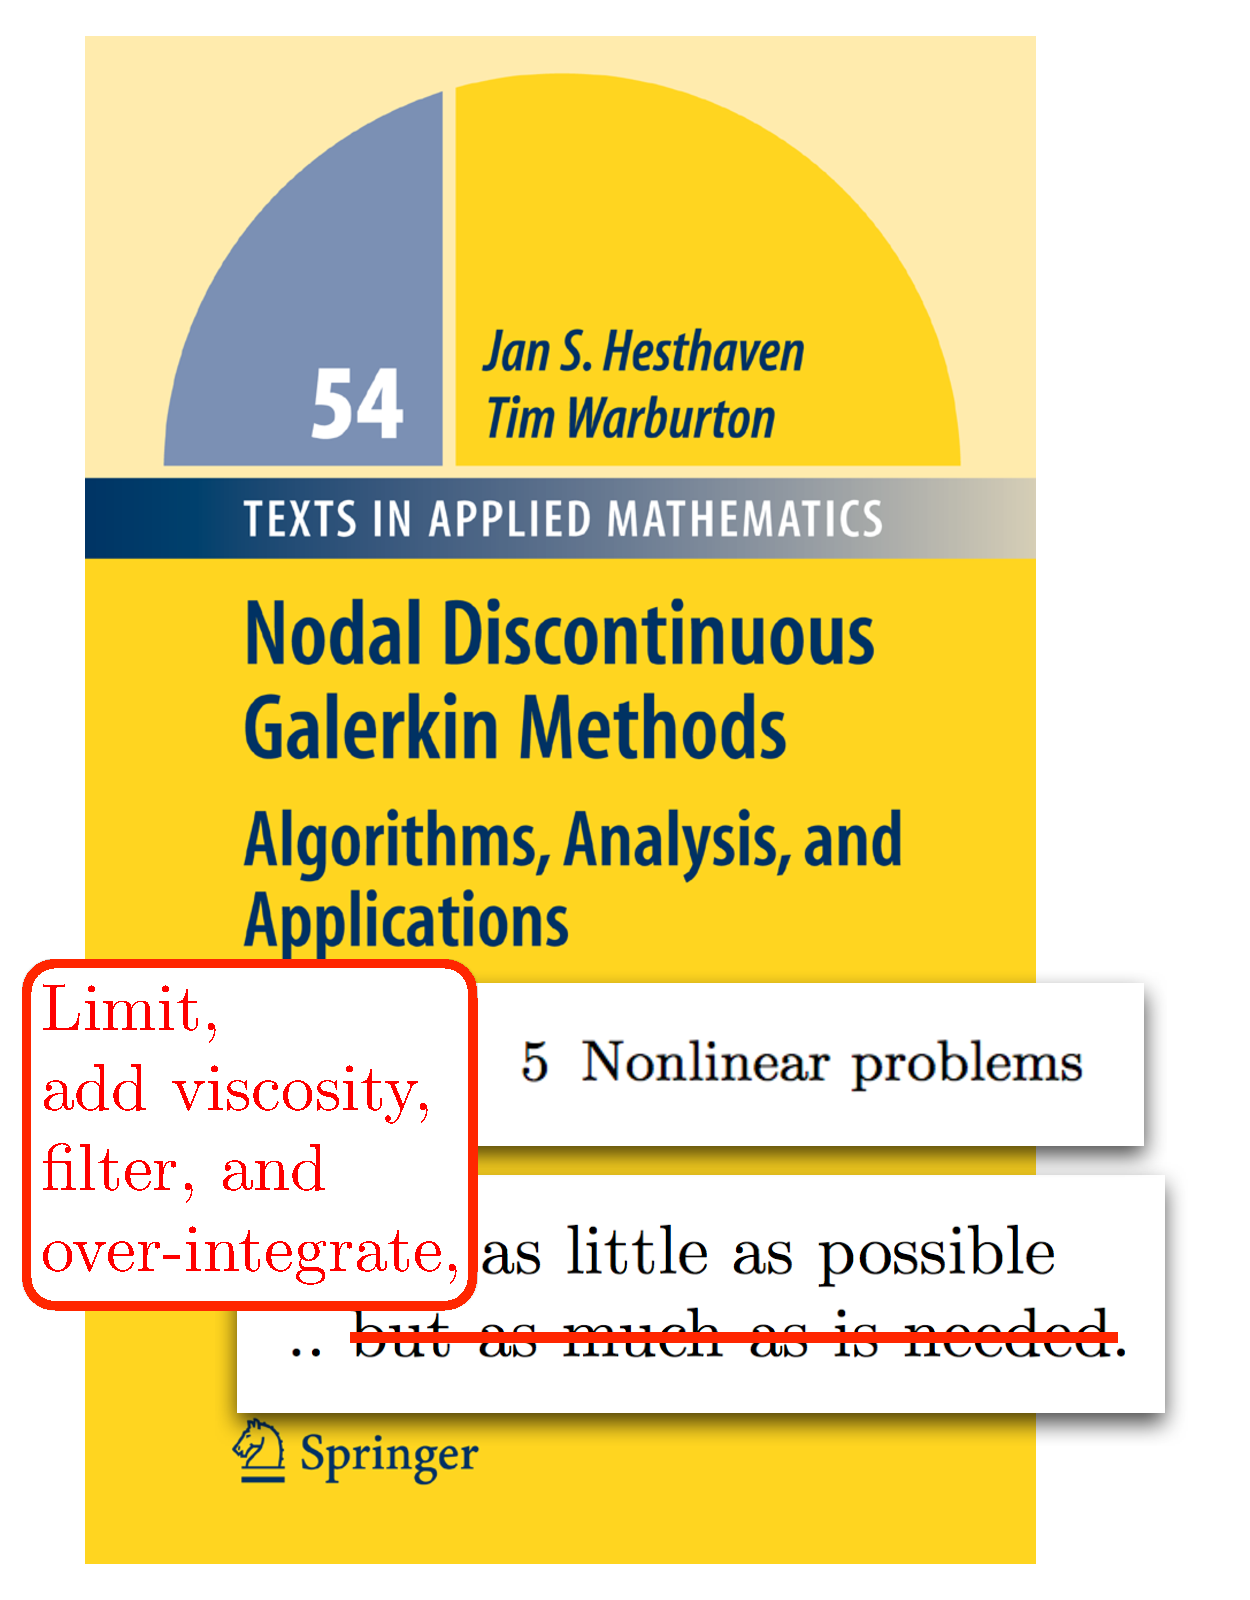
\includegraphics[width=.95\textwidth]{figs/ndgFilter2.pdf}}
%%\hspace{1em}
%\raisebox{.5em}{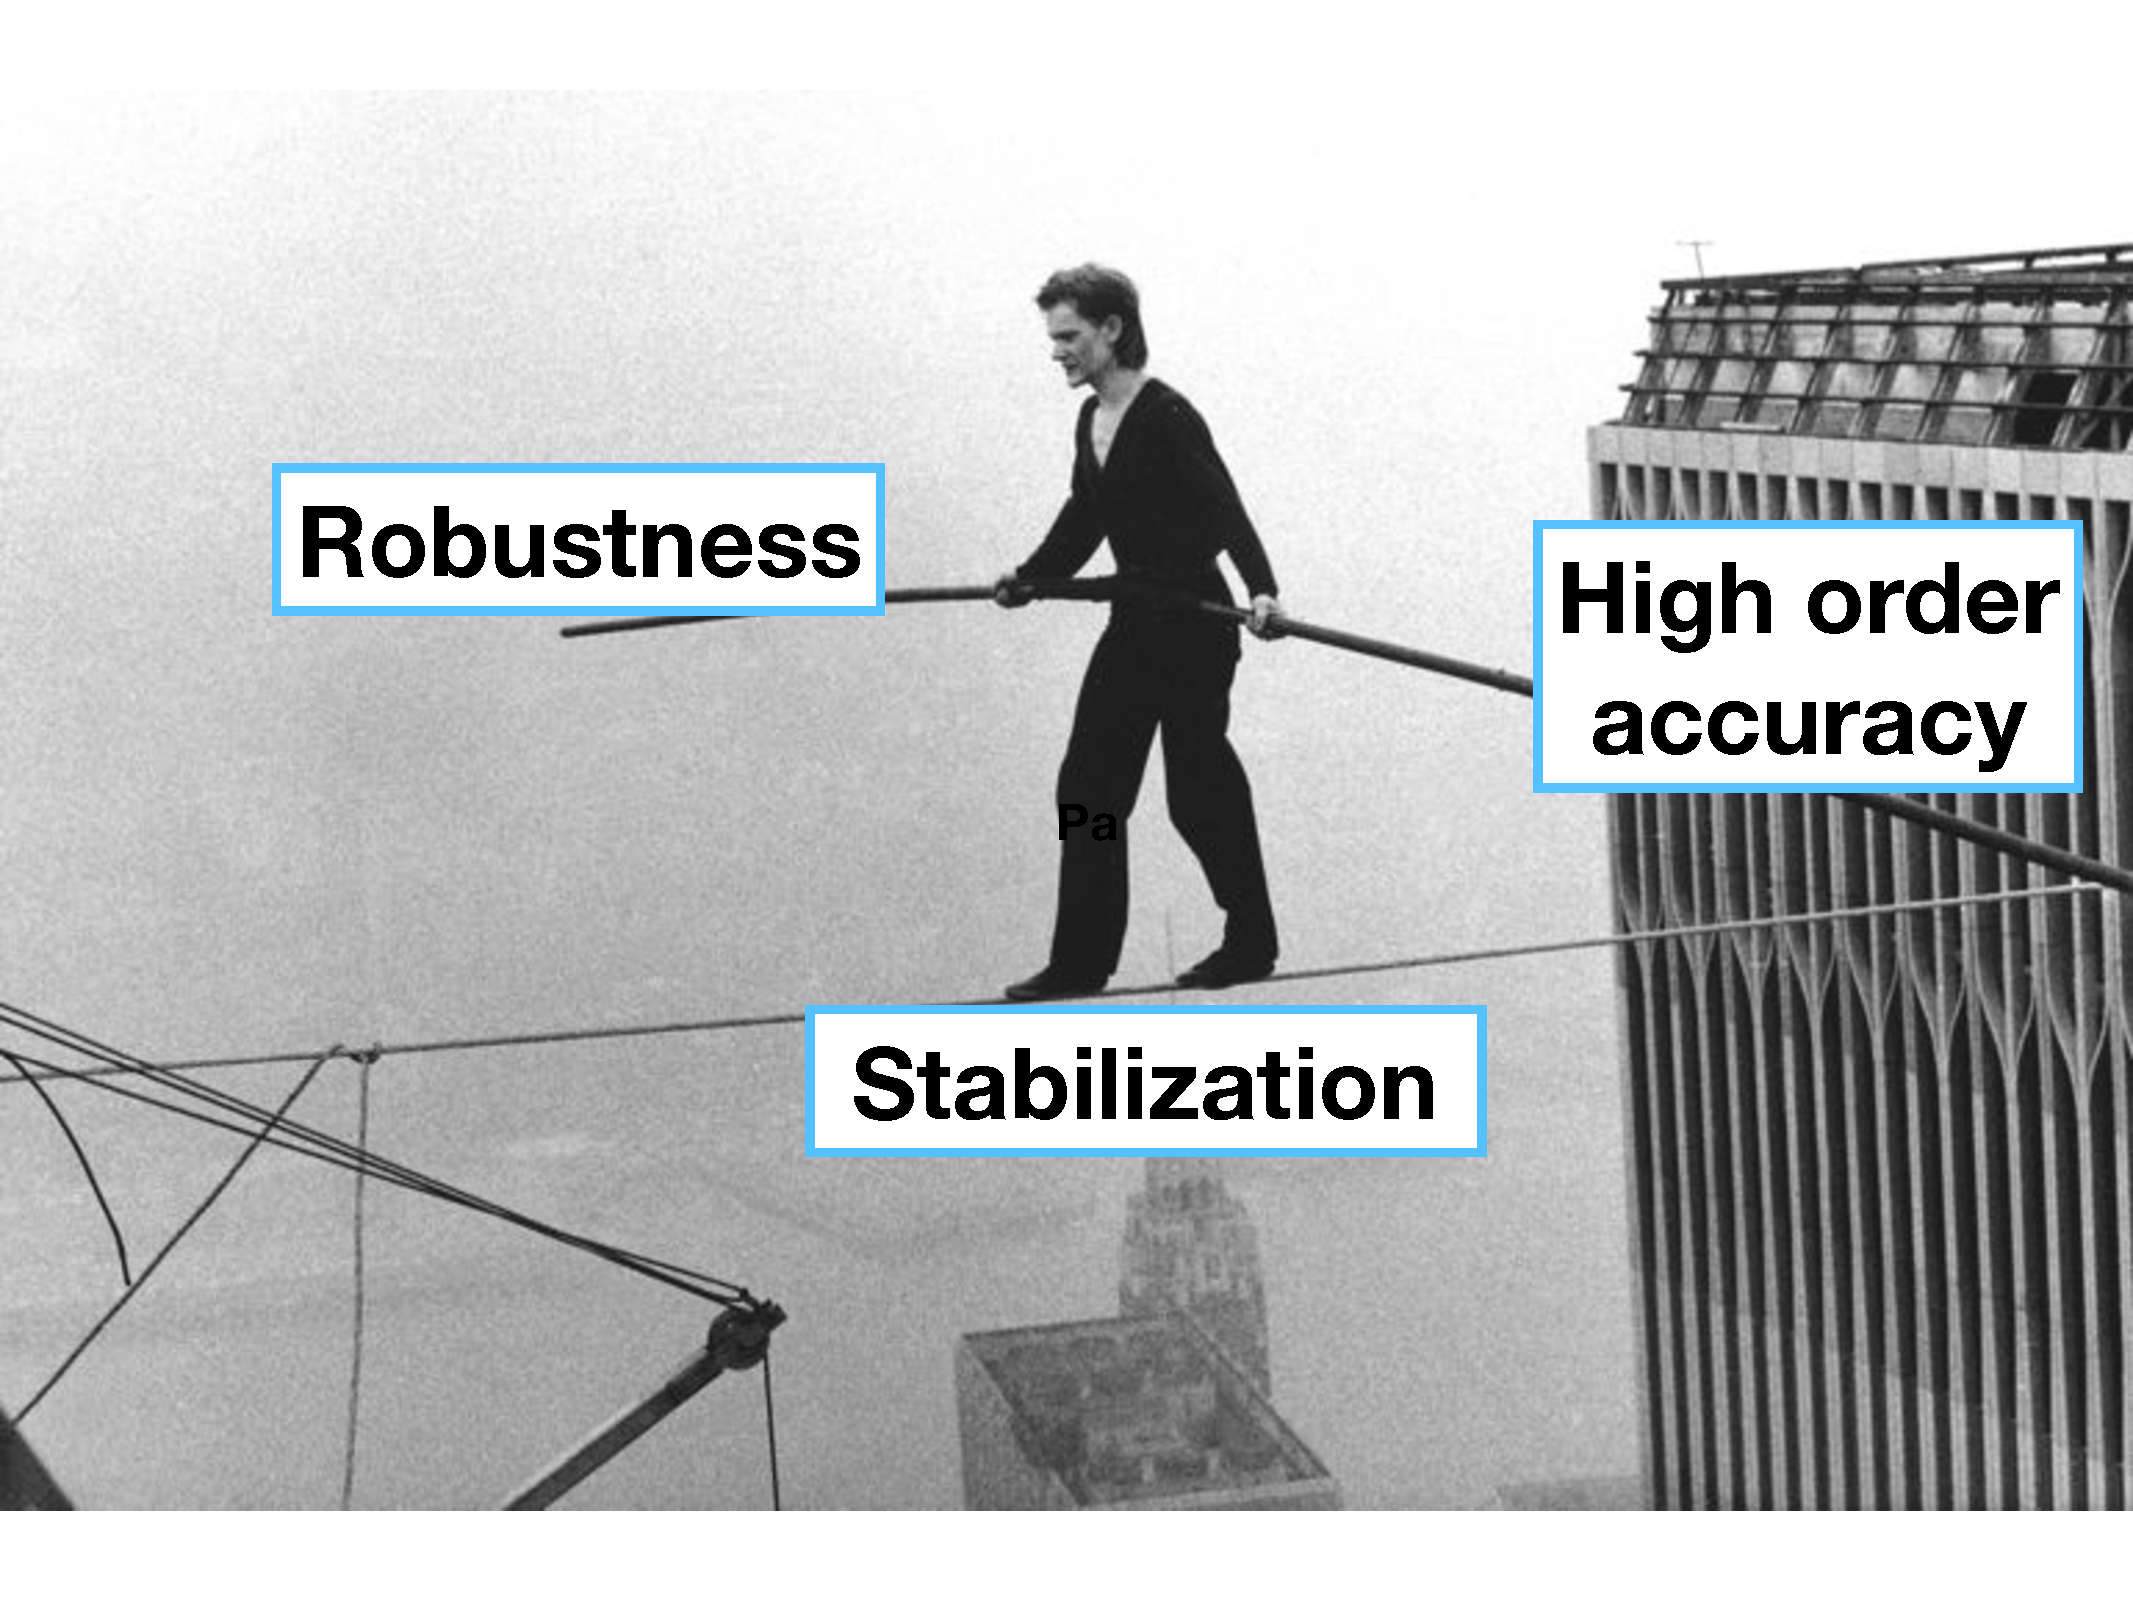
\includegraphics[width=\textwidth]{figs/balancing.pdf}}
%\caption*{\tiny Image adapted from ``Man On Wire'' (2008)}
%%\visible<5>{
\includegraphics[width=.475\textwidth]{figs/ductTape.png}}
%\end{figure}
%\end{column}
%\begin{column}{.475\textwidth}
%\begin{itemize}
%\item<1-> Aim for stability {independently} of artificial viscosity, limiters, discretization errors.
%\vspace{.75em}
%\item<1-> \textit{\note{Mechanical}} approach to stability based on algebraic properties of a discretization. 
%\vspace{.75em}
%\item<1-> Semi-discrete stability property for high order DG methods.  
%\end{itemize}
%\end{column}
%\end{columns}
%
%\let\thefootnote\relax\footnotetext{\tiny Finite volume methods: Tadmor, Chandrashekar, Ray, Svard, Fjordholm, Mishra, LeFloch, Rohde, \ldots}
%\let\thefootnote\relax\footnotetext{\tiny High order tensor product elements: Fisher, Carpenter, Gassner, Winters, Kopriva, Hindenlang, Persson, Pazner, \ldots}
%\let\thefootnote\relax\footnotetext{\tiny High order general elements: Chen and Shu, Crean, Hicken, DCDR Fernandez, Zingg, \ldots}
%}

\frame{
\frametitle{Projection-based reduced order models (ROMs)}
\vspace{-.5em}
\begin{figure}
\centering
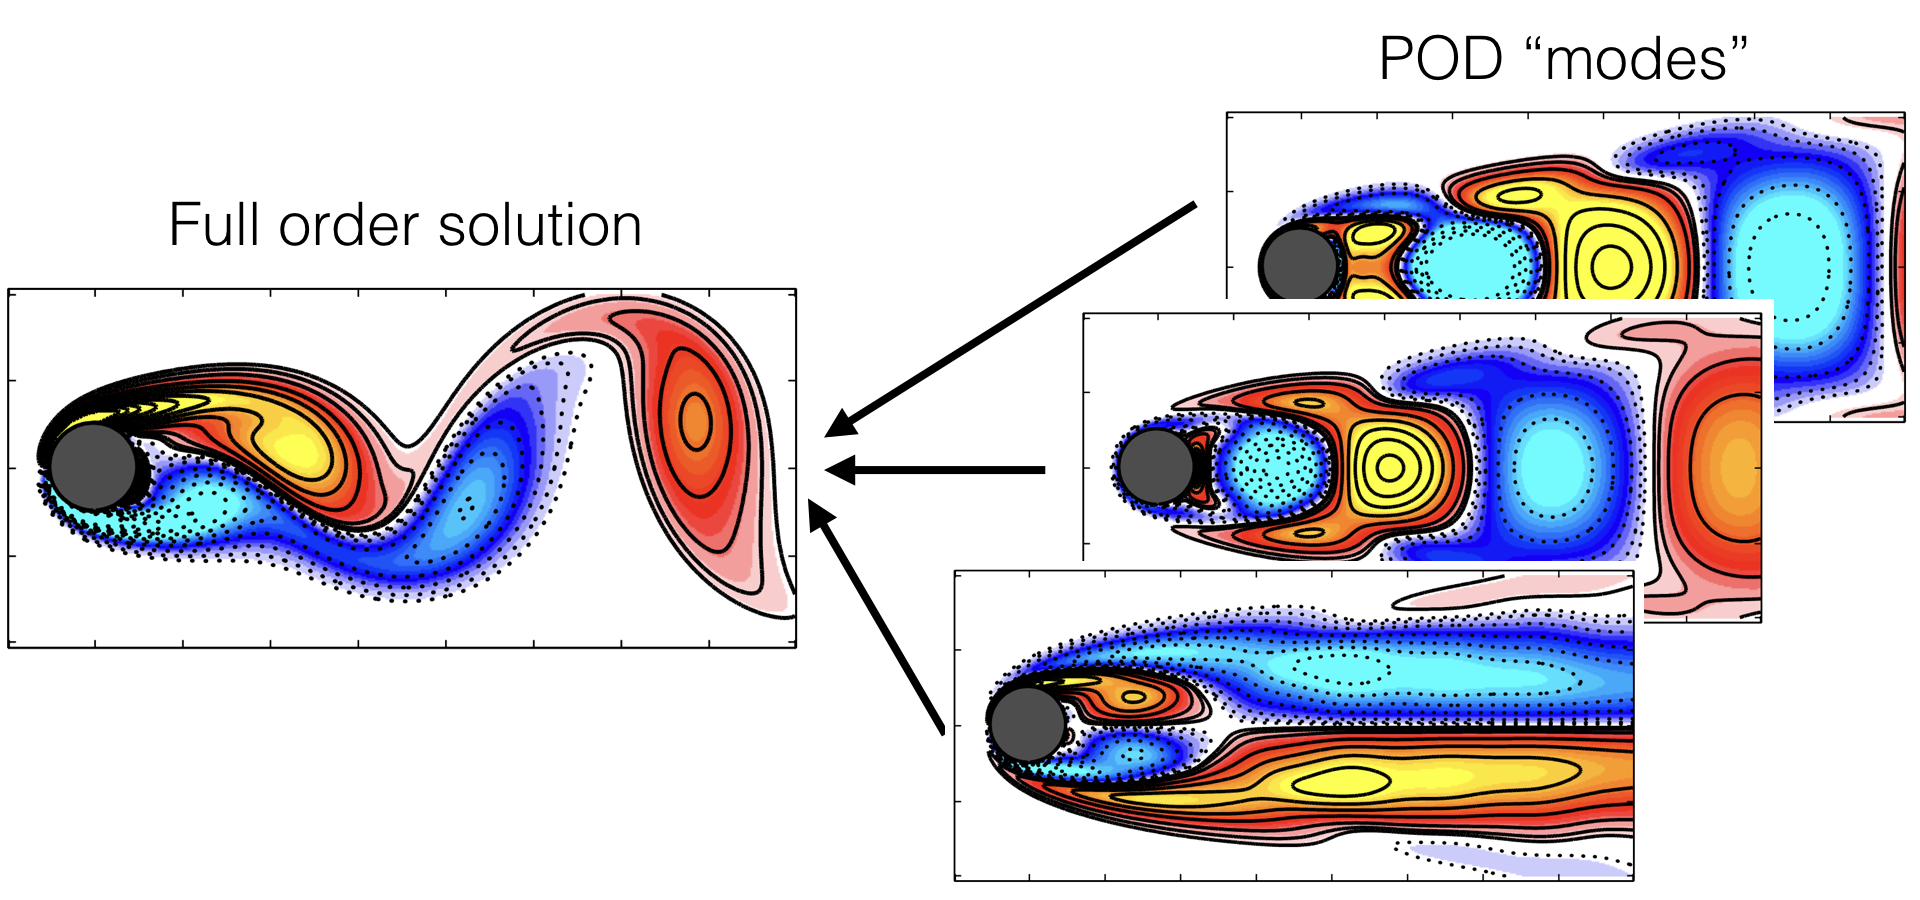
\includegraphics[width=.65\textwidth]{figs/POD_illustration.png}
\end{figure}
\vspace{-.5em}
\begin{itemize}
\item Goal: reduce cost of many-query scenarios (design space exploration).
\item \note{Offline} compute reduced basis from snapshots of full order model (FOM), cheap \note{online} phase with reduced order model (ROM).
\end{itemize} 

\uncover<2>{
\begin{center}
\minibox[frame]{Challenge: ROMs inherit FOM stability for elliptic\\
PDEs, but not for nonlinear conservation laws!}
\end{center}
}

\let\thefootnote\relax\footnotetext{\tiny Figure adapted from Brunton, Proctor, Kutz (2016), \textit{Discovering governing equations from data \ldots}.}
}

\frame{
\frametitle{Discrete instability for nonlinear PDEs}
\setcounter{subfigure}{0}
\vspace{-1em}
\begin{figure}
\begin{overprint}
\centering
\foreach \id in {1,2,3,4}{%
\only<\id>{
\captionsetup[subfloat]{width=.45\textwidth, justification=centering}
\subfloat[Exact solution]{%[$N = 7, K = 8$ (aligned mesh)]{
\makebox[.425\textwidth]{\includegraphics[width=.4\textwidth]{figs/burgersStable_\id.png}}}%
\hspace{1em}%
\subfloat[High order instability]{ %[$N = 7, K = 9$ (non-aligned mesh)]{
\makebox[.425\textwidth]{\includegraphics[width=.4\textwidth]{figs/burgersUnstable_\id.png}}}
} % only
} % foreach 
\end{overprint}
\end{figure}
\vspace{-.5em}
\begin{itemize}
\item For a larger number of modes, ROMs can blow up for under-resolved solutions of \note{nonlinear conservation laws} (shocks, turbulence).  
\vspace{.25em}
\item Instability tied to loss of the \note{chain rule} and inexact integration.  
\end{itemize}

\let\thefootnote\relax\footnotetext{\tiny Bui-Thanh, Willcox, et al.\ (2007). \textit{Goal-oriented, model-constrained optimization for reduction of large-scale systems}.}
}

\frame{
\frametitle{Entropy stability for nonlinear problems}
\vspace{-.5em}
\begin{itemize}
\item Generalizes energy stability to \note{nonlinear} systems of conservation laws (Burgers', shallow water, compressible Euler, MHD).  
\[
\pd{\bm{u}}{t} + \pd{\bm{f}(\bm{u})}{x} = 0.  
\]
\item Continuous entropy inequality: given a convex \note{entropy} function $S(\bm{u})$, entropy variables $\bm{v} = \bm{v}(\bm{u})$, and ``entropy potential'' $\psi(\bm{u})$, 
\begin{align*}
&\int_{\Omega} \bm{v}^T\LRp{\pd{\bm{u}}{t} + \pd{\bm{f}(\bm{u})}{x}} = 0, \qquad \boxed{\bm{v}(\bm{u}) = \LRu{\pd{S}{\bm{u}}}_{\bm{u}}} \\
&\Longrightarrow \int_{\Omega}\pd{S(\bm{u})}{t} + \LRu{\LRp{\bm{v}^T\bm{f}(\bm{u}) - \psi(\bm{u})}}_{-1}^1 \leq 0.
\end{align*}
\vspace{.0em}
\item Proof of entropy inequality relies on \note{chain rule}, integration by parts.  
\end{itemize}
}

\frame{
\frametitle{How is instability addressed in practice?}

\begin{overlayarea}{\textwidth}{.85\textheight}
\begin{itemize}
\item<1-> \textcolor{red}{Asymptotic} stability for \textcolor{red}{smooth} solutions (not shocks or turbulence!)
\item<3-> Common fix: \note{stabilize by regularizing} (filtering, added dissipation).  
\end{itemize}
\begin{figure}
\centering
\only<1>{
\vspace{.5em}
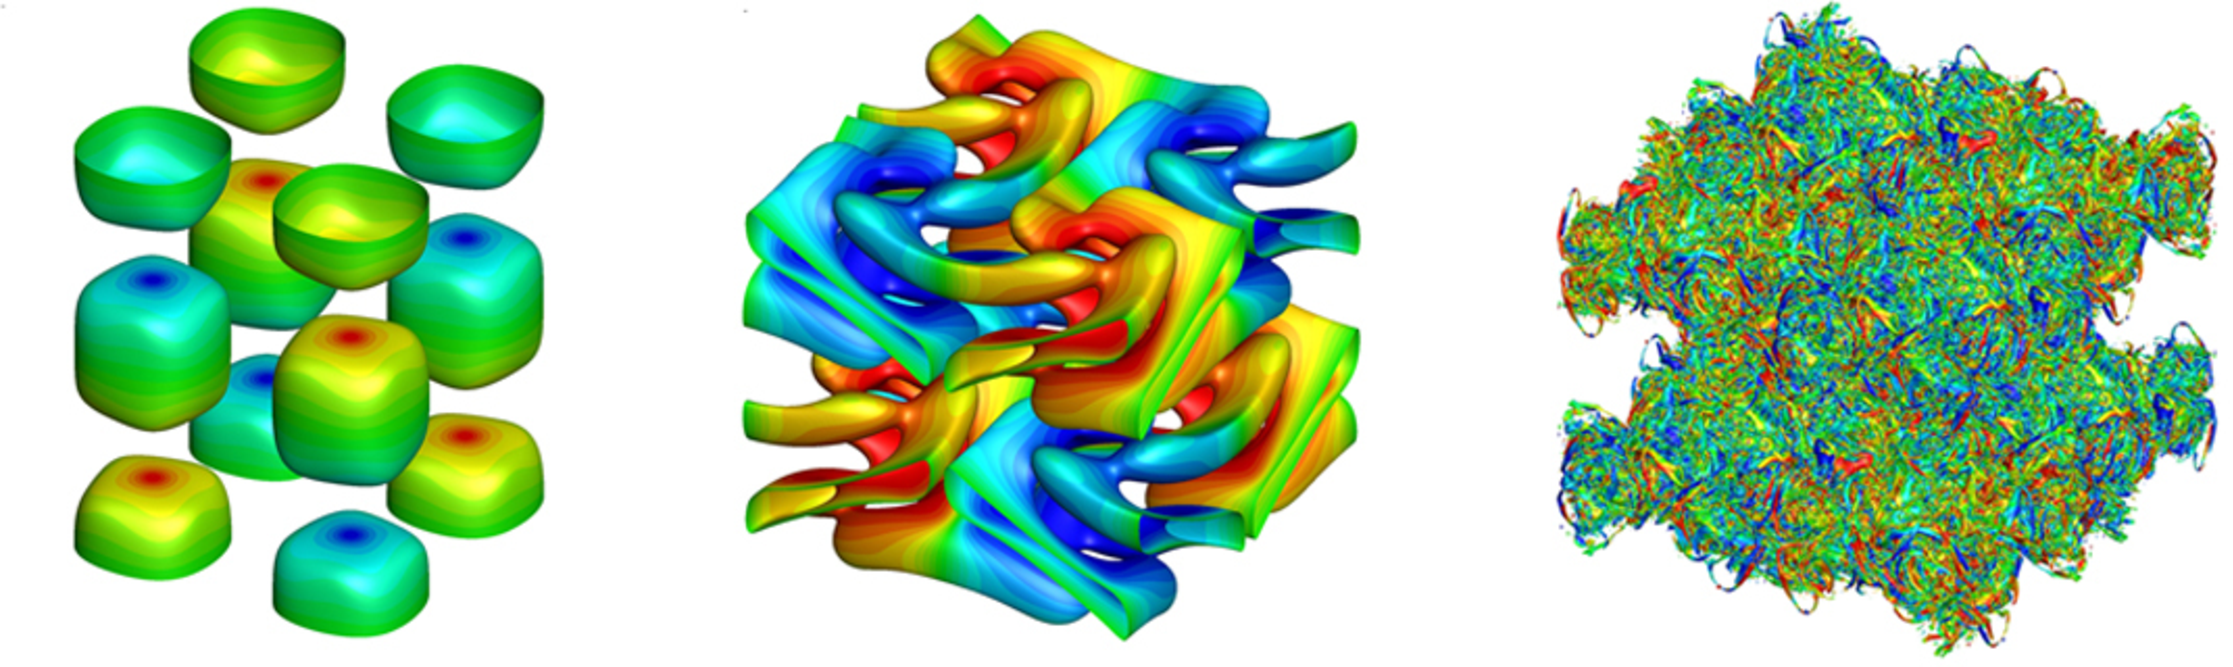
\includegraphics[width=1\textwidth]{figs/gassner_turb_01.pdf}
\caption*{Under-resolved solutions: turbulence (inviscid Taylor-Green vortex).}}
\only<2>{
\vspace{-.5em}
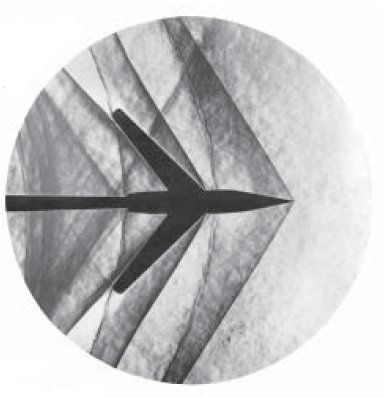
\includegraphics[width=.35\textwidth]{figs/shadowgraph.jpg}
\hspace{1em}
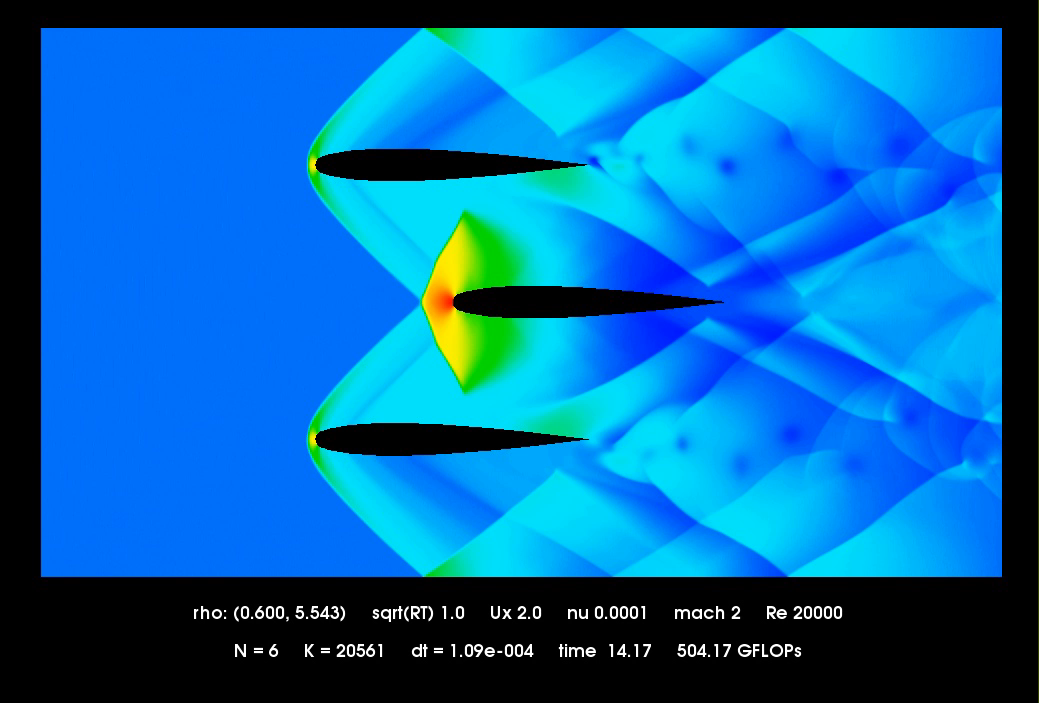
\includegraphics[width=.5\textwidth]{figs/trifoil.png}
\caption*{Under-resolved solutions: shock waves.}
}
\only<3->{
\vspace{-1em}
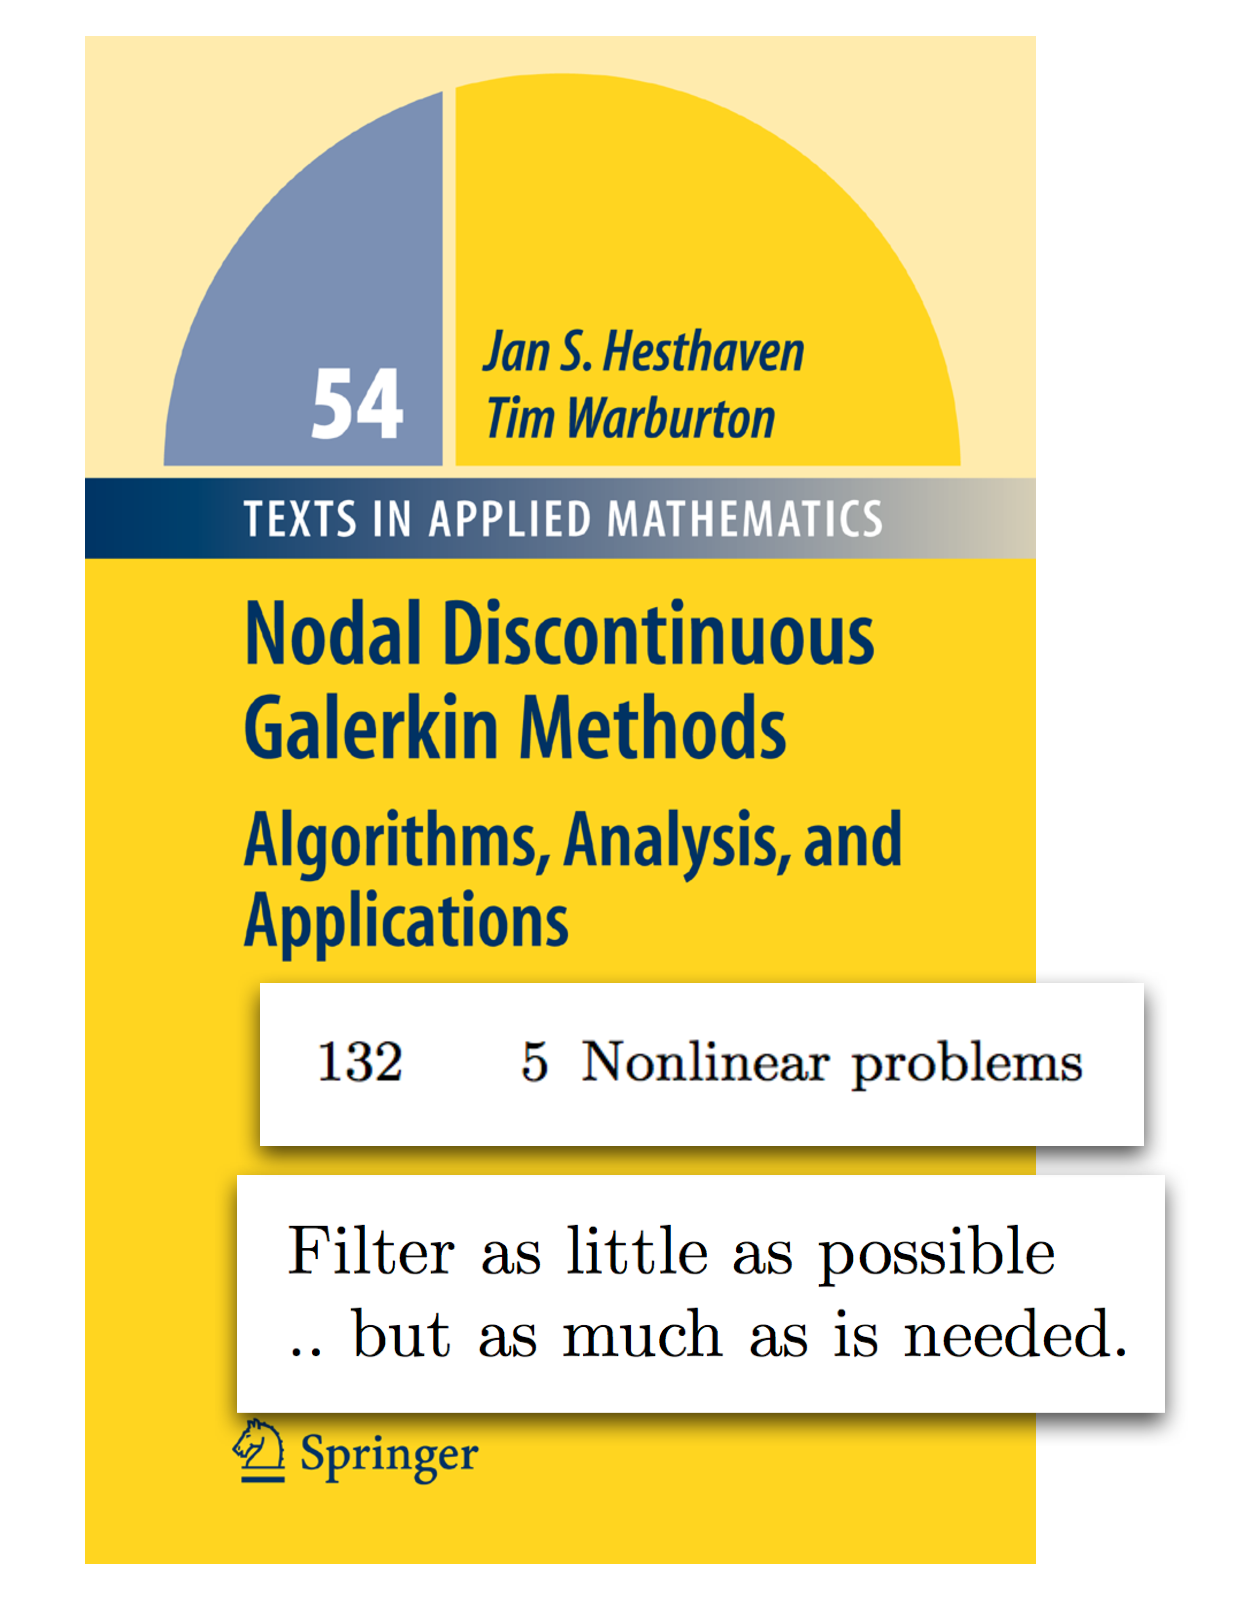
\includegraphics[width=.38\textwidth]{figs/ndgFilter.pdf}
\hspace{1em}
\visible<4>{\raisebox{2.5em}{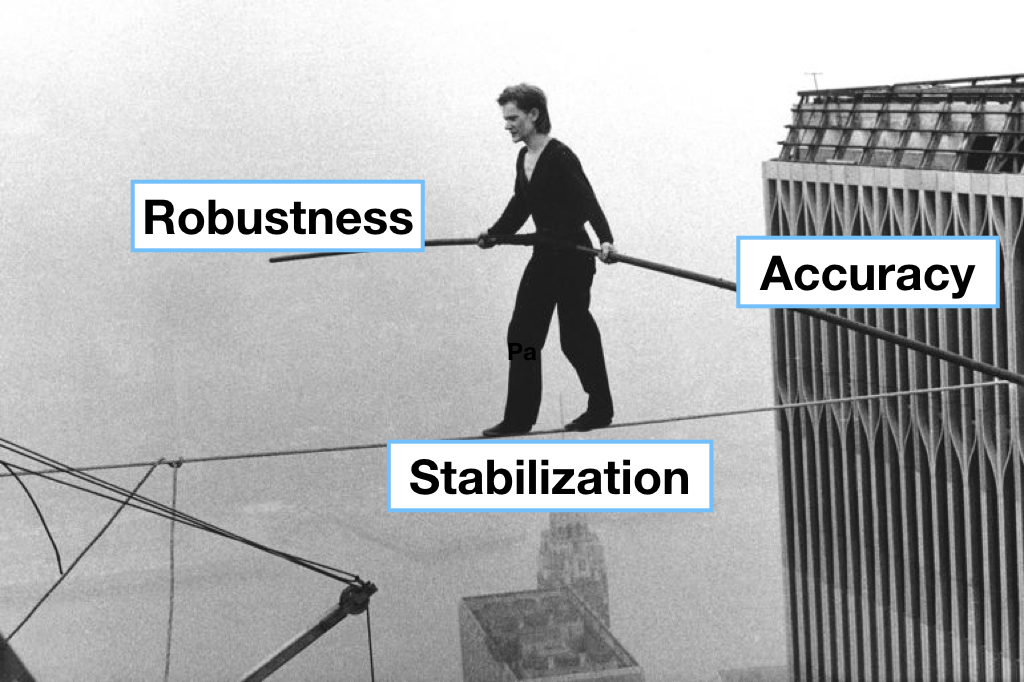
\includegraphics[width=.55\textwidth]{figs/balancing.png}}}
%\visible<5>{
\includegraphics[width=.475\textwidth]{figs/ductTape.png}}
}
\end{figure}
\end{overlayarea}
\let\thefootnote\relax\footnotetext{\tiny Figures from Beck and Gassner (2012), T.\ Warburton, \href{http://cirpwiki.info/wiki/CMS-Flow_Numerical_Methods}{\note{Coastal Inlets Research Program (CIRP)}}, ``Man on Wire'' (2008).}
}

\frame{
\frametitle{Scope of this talk, related work}

\begin{itemize}
\item Semi-discrete entropy inequality + retaining ROM accuracy.  
\vspace{1em}
\item Combinations of ideas from:
\vspace{.5em}
\begin{itemize}
\item<1-> entropy stable finite volume schemes,
\vspace{.5em}
\item<2-> high order entropy stable summation-by-parts (SBP) finite differences and nodal discontinuous Galerkin methods,
\vspace{.5em}
\item<3-> reduced order modeling and hyper-reduction.
\end{itemize}
\vspace{1em}
\item<4-> Does not address \textit{approximation issues} for transport problems!  
\end{itemize}

\let\thefootnote\relax\footnotetext{\tiny Finite volumes: Tadmor, Chandrashekar, Ray, Svard, Fjordholm, Mishra, LeFloch, Rohde, \ldots}
\let\thefootnote\relax\footnotetext{\tiny SBP: Fisher, Carpenter, Gassner, Winters, Kopriva, Hindenlang, Chen and Shu, Crean and Hicken, DCDR Fernandez, Zingg, Yamaleev, Parsani, Svard, Pazner and Persson, Wintermeyer, Bohm, Friedrich, Schnuke, \ldots.}
\let\thefootnote\relax\footnotetext{\tiny ROMs: Afkham, Ripamonti, Wang, Hesthaven (2018), Serre, Lafon, Gloerfelt, Bailly (2012), Kalashnikova, Barone, et al.\ (2014), Carlberg, Choi, Sargsyan (2018), Farhat, Chapman, Avery (2015), \ldots. }
}

\section{Starting point: an entropy stable full order model}

\frame[noframenumbering]{
\frametitle{Talk outline}

\only<1>{\tableofcontents}
\only<2>{\tableofcontents[currentsection,currentsubsection]}
}



\frame{
\frametitle{Full order model: entropy stable finite volumes}
\vspace{-.75em}
\begin{figure}
\centering
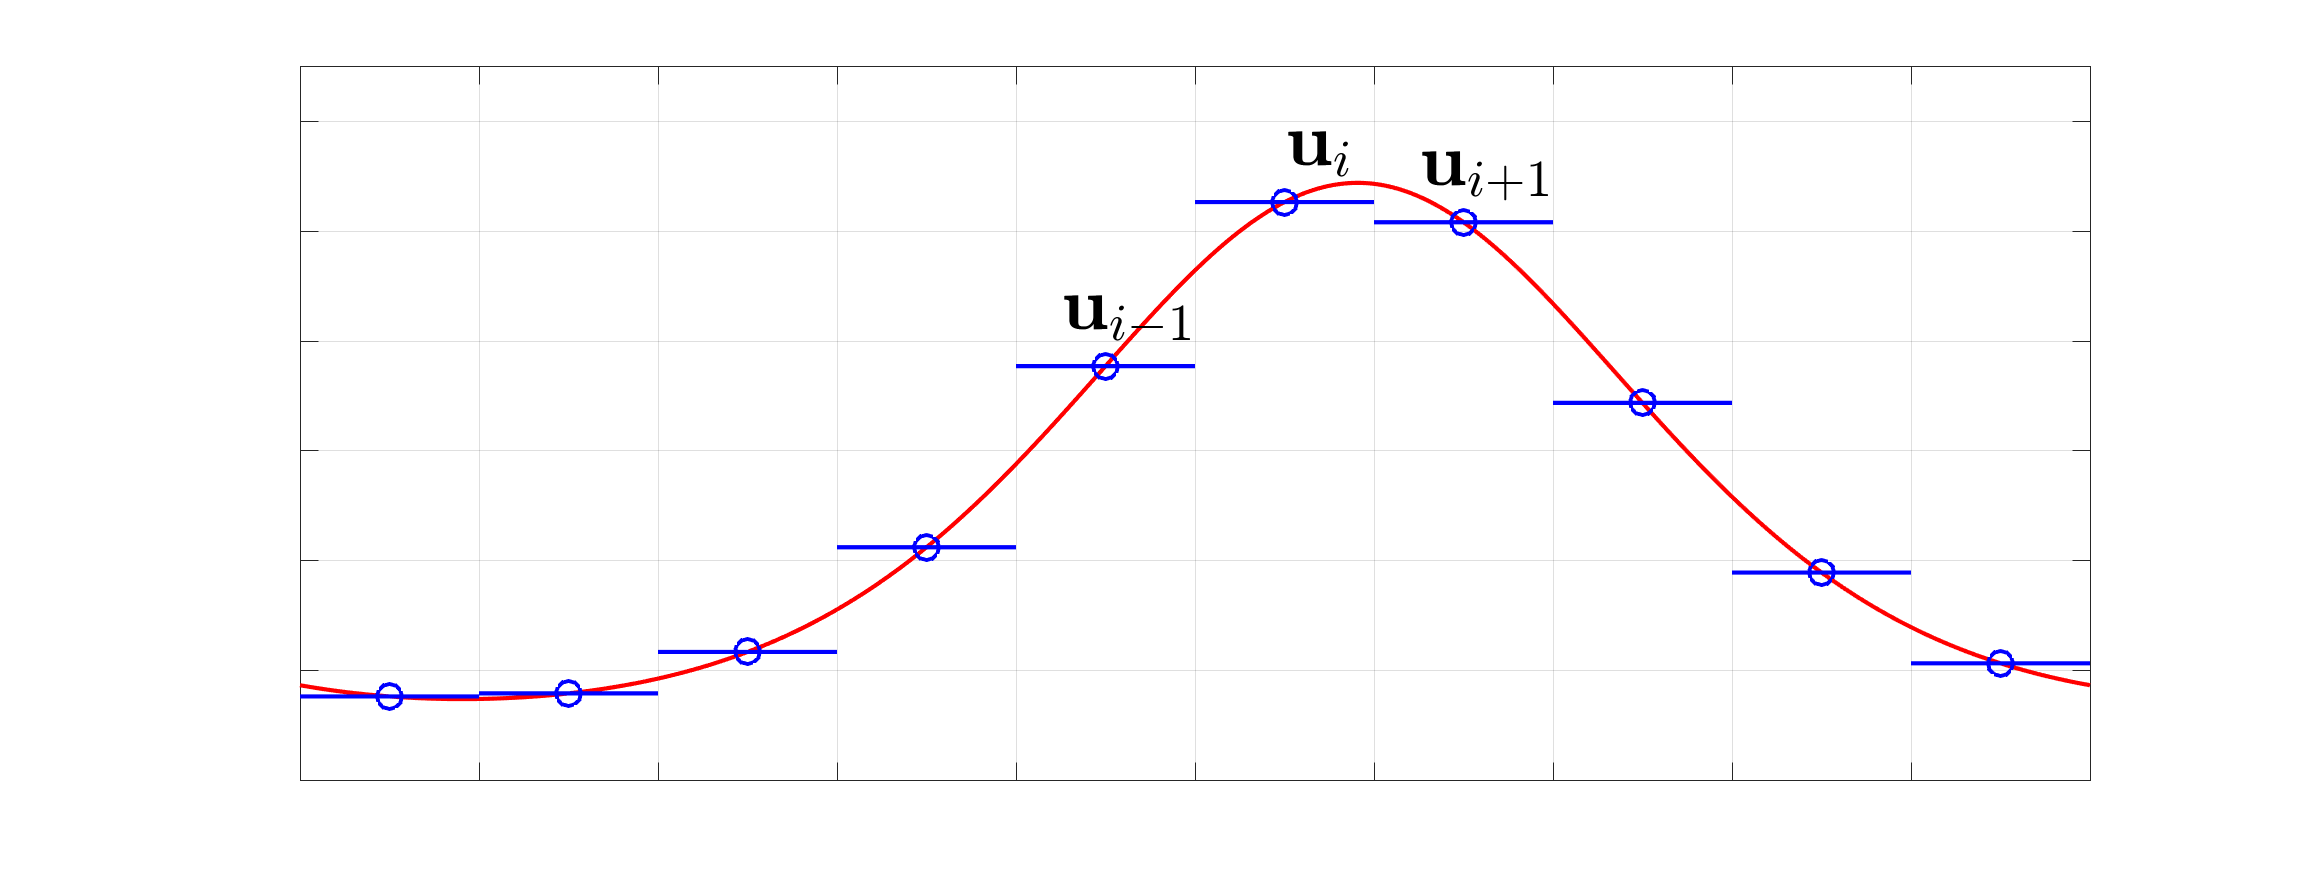
\includegraphics[width=.65\textwidth]{figs/fv_illustration.png}
\end{figure}
\vspace{-1.25em}
\begin{itemize}
\item Discretize integrated form of nonlinear conservation law
\[
\Delta x \td{\bm{u}_i}{t} + {\bm{f}_{S}(\bm{u}_{i+1},\bm{u}_i) - \bm{f}_{S}(\bm{u}_{i},\bm{u}_{i-1})} = 0.
\]
\item Matrix formulation:  let $\bm{F}_{ij} = \bm{f}_S\LRp{\bm{u}_i,\bm{u}_j}$, assume periodicity,
\[
\Delta x\td{\bm{u}}{t} + \LRp{\bm{Q}\circ \bm{F}}\bm{1}  = 0, \qquad \bm{Q} = \begin{bmatrix}
0 & 1 & & -1\\
-1 & 0 & 1 &\\
& \ddots & \ddots & 1 \\
1 & & -1  & 0
\end{bmatrix}
\]
\end{itemize}
}

\frame{
\frametitle{Recovering a semi-discrete entropy balance}
\vspace{-.5em}
\begin{itemize}
\item First, show that entropy is \textit{conserved} for the inviscid case.  Test with vector of entropy variables $\bm{v}$ 
\[
\bm{v}^T\LRp{\Delta x\td{\bm{u}}{t} + \LRp{\bm{Q}\circ \bm{F}}\bm{1}} = \bm{0}. 
\]
\item Use chain rule in time and definition of entropy variables
\[
\bm{v}^T\td{\bm{u}}{t} = \td{S(\bm{u})}{\bm{u}}^T \td{\bm{u}}{t} = \bm{1}^T \td{S(\bm{u})}{t}.
\]
\item If \note{$\bm{v}^T \LRp{\bm{Q}\circ \bm{F}}\bm{1} = 0$}, then the average entropy is conserved
\[
\Delta x \LRp{\bm{1}^T\td{S(\bm{u})}{t}} = 0.
\]
%\item Assume 
%\[
%\bm{v}^T\td{\bm{u}}{t} = \pd{S(\bm{u})}{\bm{u}}^T \td{\bm{u}}{t} = \pd{S(\bm{u})}{t} .
%\]
%\vspace{-.5em}
\end{itemize}

}

\frame{
\frametitle{Entropy conservation for the full order model}

\begin{itemize}
%\item Assume $\epsilon = 0$.  
\item Define $\bm{F}_{ij}$ using Tadmor's entropy conservative numerical flux
\begin{gather*}
\bm{f}_S(\bm{u},\bm{u}) = \bm{f}(\bm{u}), \qquad \text{(consistency)}\\
\bm{f}_S(\bm{u},\bm{v}) = \bm{f}_S(\bm{v},\bm{u}), \qquad \text{(symmetry)} \\
%,\qquad \text{(symmetry)} \\
\LRp{\bm{v}_L - \bm{v}_R}^T \bm{f}_S\LRp{\bm{u}_L,\bm{u}_R} = \psi_L - \psi_R, \qquad \text{(conservation)}.
\end{gather*}
\item Use \note{$\bm{Q} = -\bm{Q}^T$} and \note{$\bm{Q}\bm{1} = \bm{0}$} to show $\bm{v}^T\LRp{\bm{Q}\circ \bm{F}}\bm{1} = 0$.
%\[
%\bm{v}^T\LRp{\bm{Q}\circ \bm{F}}\bm{1} = 
%\only<1>{\sum_{ij} {\bm{Q}_{ij}} \bm{v}_i^T \bm{f}_S\LRp{\bm{u}_i,\bm{u}_j}}
%\only<2>{ \frac{1}{2}\sum_{ij} \note{\LRp{\bm{Q}_{ij} - \bm{Q}_{ji}}} \bm{v}_i^T \bm{f}_S\LRp{\bm{u}_i,\bm{u}_j}}
%\only<3>{ \frac{1}{2}\sum_{ij} \bm{Q}_{ij} \textcolor{red}{\LRp{\bm{v}_i - \bm{v}_j}^T \bm{f}_S\LRp{\bm{u}_i,\bm{u}_j}}}
%\only<4>{ \frac{1}{2}\sum_{ij} \bm{Q}_{ij} \LRp{\psi(\bm{u}_i) - \psi(\bm{u}_j)}}
%\only<5>{ \frac{1}{2}\LRp{\bm{\psi}^T\bm{Q}\bm{1} - \bm{1}^T\bm{Q}\bm{\psi}}}
%\only<6>{ \bm{0} \qquad \Longrightarrow \qquad \boxed{\td{S(\bm{u})}{t} = 0.}}
%\]
\begin{overlayarea}{\textwidth}{.425\textheight}
\vspace{-1em}
\begin{align*}
\bm{v}^T\LRp{\bm{Q}\circ \bm{F}}\bm{1} &= \sum_{ij} {\bm{Q}_{ij}} \bm{v}_i^T \bm{f}_S\LRp{\bm{u}_i,\bm{u}_j}\\
&= \only<1>{\frac{1}{2}\sum_{ij} \note{\LRp{\bm{Q}_{ij} - \bm{Q}_{ji}}} \bm{v}_i^T \bm{f}_S\LRp{\bm{u}_i,\bm{u}_j}}
\only<2->{\frac{1}{2}\sum_{ij} \bm{Q}_{ij} \textcolor{red}{\LRp{\bm{v}_i - \bm{v}_j}^T \bm{f}_S\LRp{\bm{u}_i,\bm{u}_j}}\\}
\only<3>{&=  \frac{1}{2}\sum_{ij} \bm{Q}_{ij} \LRp{\psi(\bm{u}_i) - \psi(\bm{u}_j)}}
\only<4>{&=  \frac{1}{2}\LRp{\bm{\psi}^T\bm{Q}\bm{1} - \bm{1}^T\bm{Q}\bm{\psi}} = \bm{0}}
%\only<5>{ \bm{0} \qquad \Longrightarrow \qquad \boxed{\td{S(\bm{u})}{t} = 0.}}
\end{align*}
\end{overlayarea}
\end{itemize}
\let\thefootnote\relax\footnotetext{\tiny Tadmor, Eitan (1987). \textit{The numerical viscosity of entropy stable schemes for systems of conservation laws. I.}}
}

\frame{
\frametitle{Entropy stability for the full order model}
\vspace{-.5em}
\begin{itemize}
\item Add appropriate \note{entropy dissipation} terms 
\begin{gather*}
\bm{v}^T\LRp{\Delta x\td{\bm{u}}{t} + \LRp{\bm{Q}\circ \bm{F}}\bm{1}  - \LRp{\text{viscous terms}}} = 0\\
\Longrightarrow \quad \Delta x \bm{1}^T \td{\bm{S}}{t} = \bm{v}^T \LRp{\text{viscous terms}} \overset{?}{\leq} 0.
\end{gather*}
\vspace{.0em}
\item Entropy is convex $\Longrightarrow$ Hessian inverse $\pd{\bm{u}}{\bm{v}}$ is SPD
\[
-\epsilon\pdn{\bm{u}}{x}{2} = -\epsilon\pd{}{x} \LRp{\pd{\bm{u}}{x}} = -\epsilon\pd{}{x}\LRp{{\pd{\bm{u}}{\bm{v}}}   \pd{\bm{v}}{x}}.
\]
Standard FEM/ROM treatment of diffusion tensor dissipates entropy.
\end{itemize}

\let\thefootnote\relax\footnotetext{\tiny Hughes, Mallet, Franca (1986). \textit{A new FE formulation for CFD: I. Sym.\ forms of the comp.\ Euler and NS equations \ldots}}
%\let\thefootnote\relax\footnotetext{\tiny Carpenter et al.\ (2014). \textit{Entropy stable spectral collocation schemes for the NS equations: discontinuous interfaces.}}
%\let\thefootnote\relax\footnotetext{\tiny Riviere and Wheeler (2000).  \textit{A discontinuous Galerkin method applied to nonlinear parabolic equations}}
}


\section{An expensive but entropy stable reduced order model}

\frame[noframenumbering]{
\frametitle{Talk outline}
\tableofcontents[currentsection,currentsubsection]
}


\frame{
\frametitle{Naive POD-Galerkin procedure}
\vspace{.5em}
\begin{itemize}
\item (Offline) compute POD basis from solution component snapshots.
\[
\bm{V} = {\begin{bmatrix} \vertbar & & \vertbar \\
\phi_1 & \ldots & \phi_N\\
\vertbar & & \vertbar
\end{bmatrix}}, \qquad \bm{u} \approx \bm{V} \bm{u}_N.
\]
\vspace{.0em}
\item (Online) Galerkin projection for coefficients $\bm{u}_N$
\[
\only<1>{{\bm{V}^T} \LRp{\Delta x\td{\LRp{\bm{V}\bm{u}_N}}{t} + \LRp{{\bm{Q}}\circ \bm{F}}\bm{1}} = 0.}
\only<2->{\Delta x{\bm{V}^T\bm{V}} \td{\bm{u}_N}{t} + \bm{V}^T \LRp{{\bm{Q}}\circ \bm{F}}\bm{1} = 0.}
%\only<2>{\underbrace{\bm{V}^T\bm{V}}_{\text{orthonormal}} \td{\bm{u}_N}{t} + \bm{V}^T \LRp{{\bm{Q}}\circ \bm{F}}\bm{1} = 0.}
%\only<3->{\td{\bm{u}_N}{t} + \bm{V}^T \LRp{{\bm{Q}}\circ \bm{F}}\bm{1} = 0.}
\]
\vspace{.0em}
\item<3-> Not discretely entropy stable!  Conservative variables are in the reduced space, entropy variables are not -- cannot test with $\bm{v}(\bm{V}\bm{u}_N)$.
\begin{gather*}
\bm{u} \in {\rm span}\LRc{\phi_1,\ldots,\phi_N}, \qquad \bm{v}(\bm{u}) \not\in {\rm span}\LRc{\phi_1,\ldots,\phi_N}.
\end{gather*}
\end{itemize}
}

\frame{
\frametitle{Entropy projection and discrete entropy stability }

\begin{itemize}
\item Entropy variables are not in ROM \textit{test space}.   Solution: test with the projection (pseudoinverse) of the entropy variables 
\begin{align*}
\LRp{\bm{V}^\dagger \bm{v}\LRp{\bm{V}\bm{u}_N}}^T\LRp{\Delta x  \bm{V}^T\bm{V}\td{\bm{u}_N}{t} + \bm{V}^T \LRp{{\bm{Q}}\circ \bm{F}}\bm{1}} = 0 
\end{align*}
\vspace{0em}
\item Projected entropy variables recover time derivative of discrete entropy 
\begin{align*}
\LRp{\bm{V}^\dagger \bm{v}\LRp{\bm{V}\bm{u}_N}}^T \bm{V}^T\bm{V}\td{\bm{u}_N}{t} &= \bm{v}\LRp{\bm{V}\bm{u}_N}^T \note{\underbrace{\LRp{\bm{V}^T\bm{V}\bm{V}^{\dagger}}^T}_{\bm{V}}} \td{\bm{u}_N}{t} \\
&= \LRu{\pd{S}{\bm{u}}}_{\LRp{\bm{V}\bm{u}_N}}^T \td{\LRp{\note{\bm{V}} \bm{u}_N}}{t} = \bm{1}^T\td{S\LRp{\bm{V}\bm{u}_N}}{t}
\end{align*}
%\vspace{0em}
%\item Entropy stability: evaluate $\bm{Q}\circ\bm{F}$ using projected entropy variables, enrich snapshots with entropy variables to ensure accuracy.
%\begin{gather*}
%\tilde{\bm{u}} = \bm{u}\LRp{\bm{V} \bm{V}^\dagger \bm{v}\LRp{\bm{V} \bm{u}_N}}, \qquad \LRp{\bm{F}}_{ij} = \bm{f}_S\LRp{\tilde{\bm{u}}_i,\tilde{\bm{u}}_j}
%\end{gather*}
\end{itemize}
}

\frame{
\begin{itemize}
\item Projected entropy variables are no longer mappings of the conservative variables.  Denote $\tilde{\bm{v}} = \bm{V}\bm{V}^\dagger \bm{v}\LRp{\bm{V}\bm{u}_N}$, then
\begin{align*}
\tilde{\bm{v}}^T \LRp{\bm{Q}\circ \bm{F}}\bm{1} &= \frac{1}{2}\sum_{ij}
\bm{Q}_{ij}\note{\LRp{\tilde{\bm{v}}_i - \tilde{\bm{v}}_j}^T\bm{f}_S\LRp{{\bm{u}}_i,{\bm{u}}_j}} \\
&\neq \frac{1}{2}\sum_{ij} \bm{Q}_{ij} \LRp{\psi(\bm{u}_i) - \psi(\bm{u}_j)}.
\end{align*}
\item Fix: evaluate $\bm{Q}\circ\bm{F}$ in terms of projected entropy variables, enrich snapshots with entropy variables to ensure accuracy.
\begin{gather*}
\tilde{\bm{u}} = \bm{u}\LRp{\bm{V} \bm{V}^\dagger \bm{v}\LRp{\bm{V} \bm{u}_N}}.%, \qquad \LRp{\bm{F}}_{ij} = \bm{f}_S\LRp{\tilde{\bm{u}}_i,\tilde{\bm{u}}_j}
\end{gather*}
\item Modified Galerkin projection ROM is discretely entropy stable  
\[
\Delta x {\bm{V}^T\bm{V}} \td{\bm{u}_N}{t} + \bm{V}^T \LRp{{\bm{Q}}\circ \bm{F}}\bm{1} = 0, \qquad \LRp{\bm{F}}_{ij} = \bm{f}_S\LRp{\tilde{\bm{u}}_i,\tilde{\bm{u}}_j}
\]
\end{itemize}
}

\section{Reducing nonlinear costs: entropy stable hyper-reduction}

\frame[noframenumbering]{
\frametitle{Talk outline}
\tableofcontents[currentsection,currentsubsection]
}

\frame{
\frametitle{Evaluating nonlinear ROM terms dominates costs}
\vspace{-.75em}
\begin{center}
Problem: cost of evaluating ROM nonlinear terms scales with\\
\note{number of grid points (squared)}!  No improvement over full order model.
\[
{\tilde{\bm{u}} = \note{\bm{u}}\LRp{\bm{V} \bm{V}^\dagger \note{\bm{v}}\LRp{\bm{V} \bm{u}_N}}}, \qquad \LRp{{\bm{Q}}\circ \note{\bm{F}}}\bm{1} 
\]
\end{center}
\vspace{-1em}
\uncover<2>{
\begin{columns}
\begin{column}{.55\textwidth}
\begin{itemize}
\item \note{Hyper-reduction} reduces costs by approximating nonlinear evaluations.  
\begin{align*}
&\bm{V}^T\bm{g}(\bm{V}\bm{u}_N) \approx\\
&\underbrace{\bm{V}(\mathcal{I},:)^T}_{\text{sampled rows}}\bm{W}\bm{g}(\bm{V}(\mathcal{I},:)\bm{u}_N)
\end{align*}
%\vspace{1.5em}
\item Examples: gappy POD, DEIM, empirical cubature, ECSW, \ldots
\end{itemize}
\end{column}
}
\begin{column}{.45\textwidth}
\begin{figure}
%\centering
\begin{overlayarea}{\textwidth}{.5\textheight}
\only<1>{
\includegraphics[width = .8\textwidth]{figs/hyperreduc_illustration0.png}}
\only<2>{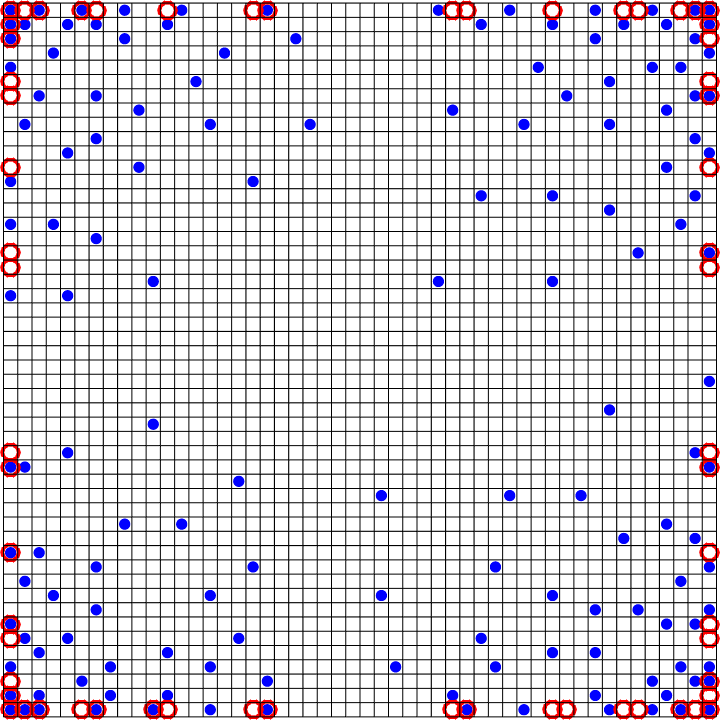
\includegraphics[width = .8\textwidth]{figs/hyperreduc_illustration.png}}
\end{overlayarea}
\end{figure}
\end{column}
\end{columns}

\let\thefootnote\relax\footnotetext{\tiny Hernandez et al., An et al., Bui/Willcox, Chantarantabut /Sorensen, Drmac/Gugercin, Farhat et al.\, Patera/Yano, \ldots}
}

\frame{
\frametitle{Entropy stability and standard hyper-reduction}

\begin{itemize}
\item How to hyper-reduce $\LRp{\bm{Q}\circ \bm{F}}$?  Construct a \textit{sampled} matrix $\bm{Q}_s$ from $\bm{Q}$.  Need \note{$\bm{Q}_s = -\bm{Q}_s^T$} and \note{$\bm{Q}_s\bm{1} = \bm{0}$} for entropy stability.
\vspace{2em}
\item Options: sub-sample rows and columns of full matrix $\bm{Q}$ or approximate $\bm{Q}$ by weighted sum of local skew matrices $\bm{Q}_e$.  
\[
\bm{Q} = \sum_{e=1}^K \bm{Q}_e \approx \bm{Q}_s = \sum_{e = 1}^K \bm{w}_e \bm{Q}_e, \qquad \bm{w} \text{ sparse}.
\]
\uncover<2->{Problems: either \note{$\bm{Q}_s$ loses skew-symmetry} or \note{$\bm{Q}_s\bm{1}\neq \bm{0}$}.}
%\vspace{1.5em}
%\item<5-> Project $\bm{Q}$ onto reduced basis $\bm{V}^T\bm{Q} \bm{V}$.
\end{itemize}

\let\thefootnote\relax\footnotetext{\tiny Patera and Yano (2017). \textit{An LP empirical quadrature procedure for parametrized functions}.}
}


\frame{
\frametitle{Two-step hyper-reduction: compress and project}
%\begin{overlayarea}{\textwidth}{\textheight}
%\vspace{1em}
\begin{itemize}
\item Step 1: construct a \textit{modal} $\bm{Q}$ using an expanded ``test'' basis $\bm{V}_t$
\[
\bm{V}_t^T\bm{Q}\bm{V}_t, \qquad \bm{V}_t = {\rm orth}\LRp{
\begin{bmatrix} 
\bm{V} & \bm{1}
\end{bmatrix}}
\]
%\vspace{1em}
\item Step 2: determine modal coefficients using hyper-reduced quadrature.  
%\item<2-> Compute \note{empirical cubature} points + projection for $\bm{Q}_s$
\begin{gather*}
\bm{W}_{ij} = w_{ii}\delta_{ij}, \\%\quad \text{ (diagonal weighting matrix)} \\
\bm{M}_t = \bm{V}_t(\mathcal{I},:)^T\bm{W}\bm{V}_t(\mathcal{I},:), \\
\bm{P}_t = \bm{M}_t^{-1}\bm{V}_t(\mathcal{I},:)^T\bm{W}.%, \qquad \text{ discrete projection}
%\bm{Q}_s = \bm{P}_t^T \LRp{\bm{V}_t^T\bm{Q}\bm{V}_t} \bm{P}_t. 
\end{gather*}
$\bm{P}_t$ is a weighted orthogonal projection onto the test basis.  %(can also use Gappy POD).
%\item<2-> Compression + sampling ensure $\bm{Q}_t\bm{1} = 0$ and $\bm{Q}_t = -\bm{Q}_t^T$ (on periodic domains) for entropy stability.
%\[
%\underbrace{\bm{V}(\mathcal{I},:)^T\bm{W}\bm{V}(\mathcal{I},:)}_{\bm{M}_N} \td{\bm{u}_N}{t} + \bm{V}(\mathcal{I},:)^T \LRp{\bm{Q}_t\circ \bm{F}_S}\bm{1} = 0.
%\]
\vspace{1em}
\item Step 3: let $\bm{Q}_s = \bm{P}_t^T\LRp{\bm{V}_t^T\bm{Q}\bm{V}_t}\bm{P}_t$.  Note $\bm{Q}_s = -\bm{Q}_s^T$ and $\bm{Q}_s\bm{1} = \bm{0}$!
\end{itemize}
%\end{overlayarea}

\let\thefootnote\relax\footnotetext{\tiny Hernandez, Caicedo, Ferrer (2017).  \textit{Dimensional hyper-reduction of nonlinear finite element models via empirical cubature.}}
%\let\thefootnote\relax\footnotetext{\tiny Everson, Sirovich (1995).  \textit{Karhunen--Loeve procedure for gappy data.}}
}

\frame{
\begin{itemize}
\item Problem: modes $\bm{V}_t$ may sample $\bm{Q}\bm{V}$ very poorly, e.g., $\bm{V}_t^T\bm{Q}\bm{V}_t\approx \bm{0}$!
\vspace{-1.5em}
\begin{figure}
\centering
\subfloat[\scriptsize Shock snapshots]{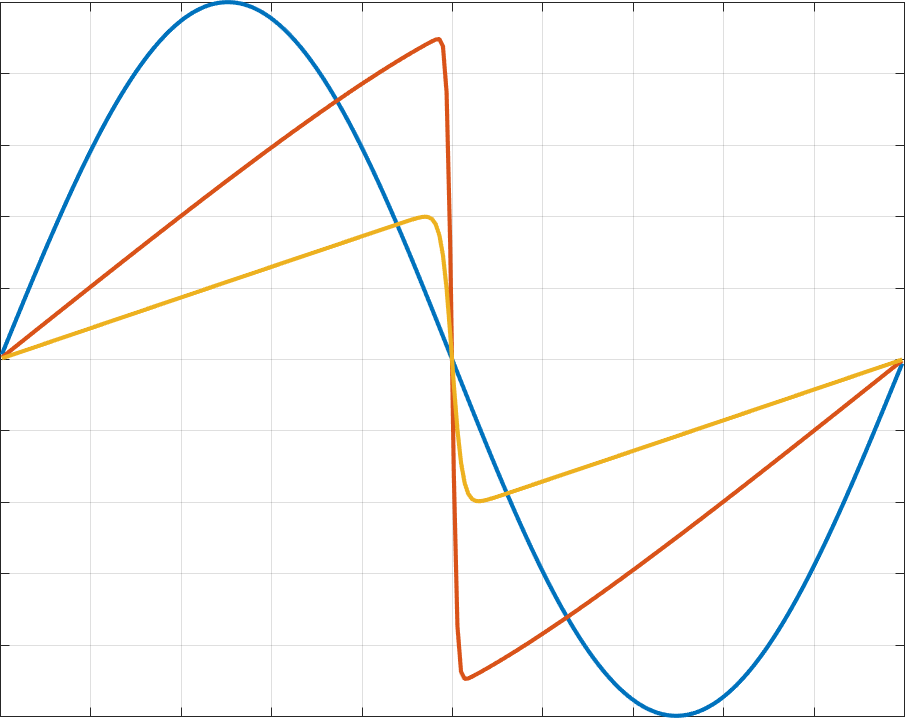
\includegraphics[width=.3\textwidth]{figs/burg_snaps.png}}
\hspace{.1em}
\subfloat[\scriptsize Modes (columns of $\bm{V}$)]{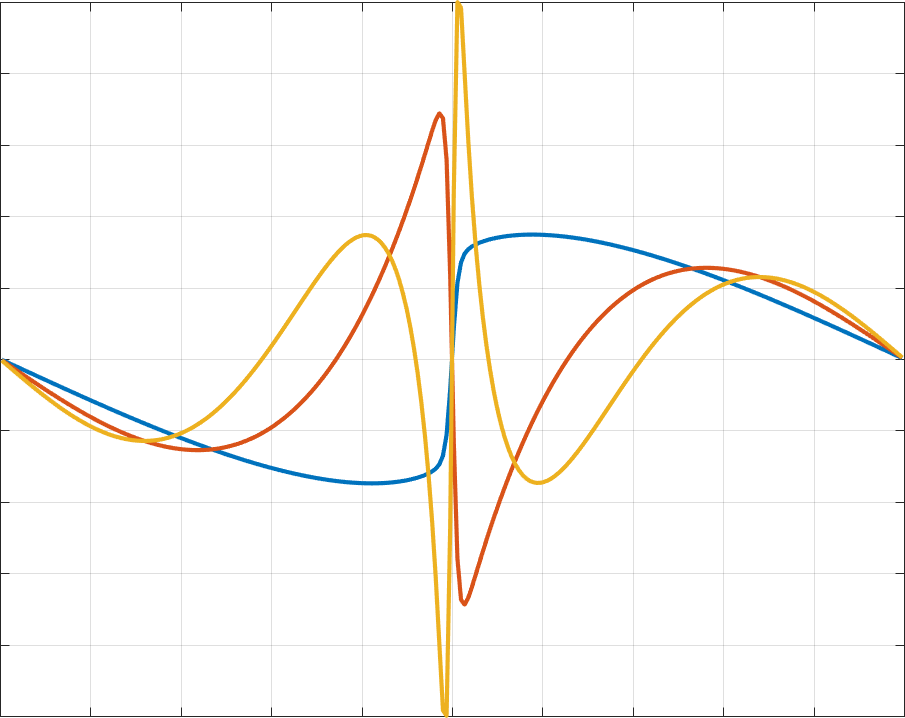
\includegraphics[width=.3\textwidth]{figs/burg3modes.png}}
\hspace{.1em}
\subfloat[\scriptsize Mode derivatives $\bm{Q}\bm{V}$]{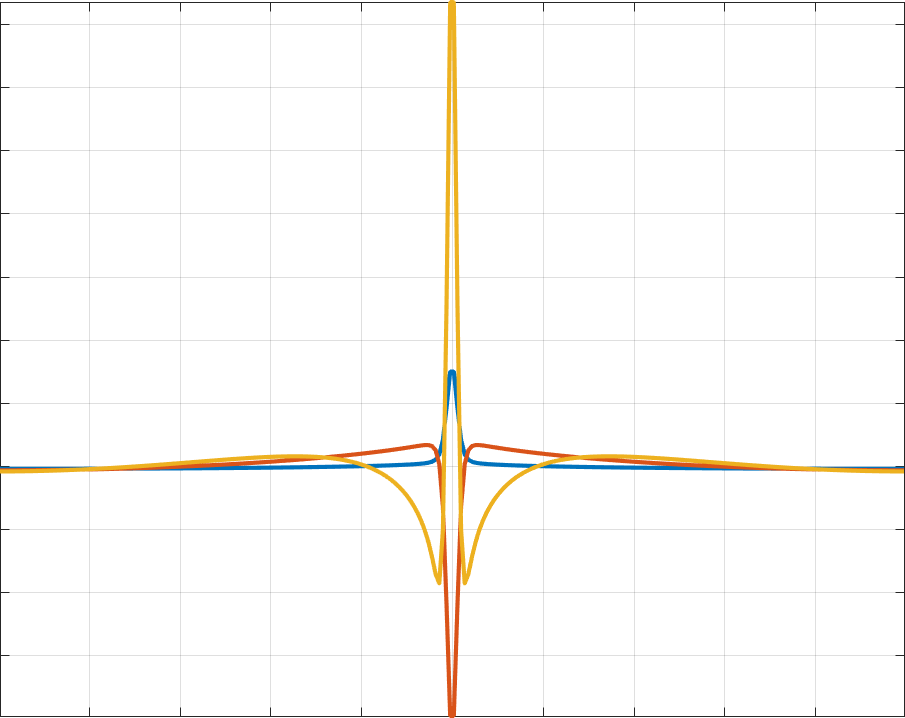
\includegraphics[width=.3\textwidth]{figs/burg3modes_diff.png}}
\end{figure}
\vspace{.5em}
\item Fix: expand basis $\bm{V}_t$ with ``least squares'' test functions
\begin{gather*}
\bm{V}_t = {\rm orth}\LRp{
\begin{bmatrix} 
\bm{V} & \bm{1} & \bm{Q}\bm{V} 
\end{bmatrix}}, \qquad
\bm{V}_t^T\bm{Q}\bm{V}_t \in \mathbb{R}^{(2N+1) \times (2N+1)}. %\mathbb{R}^{(d+1)N+1 \times (d+1)N+1}.
\end{gather*}
$\bm{V}_t^T\bm{Q}\bm{V}_t$ is accurate, skew-symmetric, and exact for constants.
\end{itemize}

\let\thefootnote\relax\footnotetext{\tiny Carlberg, Barone, Antil (2017).  \textit{Galerkin v. least-squares Petrov--Galerkin projection in nonlinear model reduction.}}
}

%\frame{
%\frametitle{Hyper-reduction through empirical cubature}
%
%\begin{itemize}
%%Reduced operator $\tilde{\bm{Q}}_N$ is skew-symmetric and satisfies $\tilde{\bm{Q}}_N\bm{1} = 0$.
%%\item Greedy algorithm for  approx.\ of $\int \phi_i(\bm{x}) \phi_j(\bm{x})$.  
%
%\let\thefootnote\relax\footnotetext{\tiny An, Kim, James (2009).  \textit{Optimizing cubature for efficient integration of subspace deformations}.}
%\let\thefootnote\relax\footnotetext{\tiny Hernandez, Caicedo, Ferrer (2017).  \textit{Dimensional hyper-reduction of nonlinear finite element models via empirical cubature.}}
%}

\frame{
\frametitle{Summary: entropy stable ROMs on periodic domains}

%\note{Summarize here}

\begin{itemize}
\item Entropy stable ROM using \textit{projected} entropy variables.  
\vspace{1em}
\item Two-step hyper-reduction of $\LRp{\bm{Q}\circ \bm{F}}$: compress and project
\begin{itemize}
\item Compress $\bm{Q}$ onto expanded test basis spanning $\bm{1}$, $\bm{Q}\bm{V}$.
\item Project hyper-reduced point values to modes of test basis 
\[
\bm{Q}_s = \bm{P}_t^T\LRp{\bm{V}_t^T\bm{Q}\bm{V}_t}\bm{P}_t
\]
%Reduced $\bm{Q}_s$ satisfies $\bm{Q}_s\bm{1} = \bm{0}$ and $\bm{Q}_s = -\bm{Q}_s^T$.
\end{itemize}
%\vspace{1em}
\item Entropy stable reduced order model with hyper-reduction:
\[
{\bm{V}(\mathcal{I},:)^T\bm{W}\bm{V}(\mathcal{I},:)} \td{\bm{u}_N}{t} + \bm{V}(\mathcal{I},:)^T \LRp{\bm{Q}_s\circ \bm{F}}\bm{1} = 0,
\]
where $\bm{P}$ is the hyper-reduced projection onto POD modes and
\begin{gather*}
%\underbrace{\bm{V}(\mathcal{I},:)^T\bm{W}\bm{V}(\mathcal{I},:)}_{\bm{M}_N} \td{\bm{u}_N}{t} + \bm{V}(\mathcal{I},:)^T \LRp{\bm{Q}_s\circ \bm{F}_S}\bm{1} = 0.
%{\bm{V}(\mathcal{I},:)^T\bm{W}\bm{V}(\mathcal{I},:)} \td{\bm{u}_N}{t} + \bm{V}(\mathcal{I},:)^T \LRp{\bm{Q}_s\circ \bm{F}}\bm{1} = 0,\\
{\bm{F}}_{ij} = \bm{f}_S\LRp{\tilde{\bm{u}}_i,\tilde{\bm{u}}_j}, \quad \tilde{\bm{u}} = \bm{u}\LRp{\bm{V}(\mathcal{I},:)\bm{P} \bm{v}\LRp{\bm{V}\bm{u}_N}},
%\LRp{\bm{V}(\mathcal{I},:)^T\bm{W}\bm{V}(\mathcal{I},:)}^{-1}{\bm{V}(\mathcal{I},:)^T\bm{W}}.
\end{gather*}
\end{itemize}
}

\frame{
\frametitle{Non-periodic boundary conditions}

\begin{itemize}
%\item Non-periodic domains: full order matrix $\bm{Q}$ is \textit{nearly} skew-symmetric
%\[
%\bm{Q} = \bm{S} + \bm{B}, \qquad \bm{S} = \begin{bmatrix} 
% 0& 1 & 0\\
%-1& 0 &1\\
%0& -1 & 0
%\end{bmatrix}, \qquad \bm{B} = \begin{bmatrix} -1 & &\\
%&0&\\
%&&1
%\end{bmatrix}
%\]
\item Treat boundary conditions weakly using ``hybridized'' summation-by-parts (SBP) operators and numerical flux.  
\vspace{1em}
\item Can add entropy-dissipative penalization terms (e.g., Lax-Friedrichs).
%\[
%\bm{Q}_N = \begin{bmatrix}
%\bm{Q}-\bm{Q}^T & \bm{E}^T\bm{B}\\
%-\bm{B}\bm{E} & 
%\end{bmatrix}
%\]
\vspace{1em}
\item Let $\bm{V}_f$ be the surface interpolation matrix.  Entropy stability requires a weak SBP property for surface quadrature weights $\bm{w}_f$ 
\begin{align*}
\bm{V}_t^T \bm{Q}_x^T\bm{1} &= \bm{V}_f^T \LRp{\bm{n}_x \circ \note{\bm{w}_f}},\\
\bm{V}_t^T \bm{Q}_y^T\bm{1} &= \bm{V}_f^T \LRp{\bm{n}_y \circ \note{\bm{w}_f}}.
\end{align*}
Enforce conditions using constrained LP hyper-reduction.
\end{itemize}

\let\thefootnote\relax\footnotetext{\tiny Patera and Yano (2017). \textit{An LP empirical quadrature procedure for parametrized functions}.}
\let\thefootnote\relax\footnotetext{\tiny Chan (2018). \textit{On discretely entropy conservative and entropy stable discontinuous Galerkin methods.}}
\let\thefootnote\relax\footnotetext{\tiny Chan (2019). \textit{Skew-symmetric entropy stable modal discontinuous Galerkin formulations}.}
}

\section{Numerical experiments}

\frame[noframenumbering]{
\frametitle{Talk outline}
\tableofcontents[currentsection,currentsubsection]
}




\frame{
\frametitle{Numerical results: 1D Euler with reflective BCs + shock}
\setcounter{subfigure}{0}
\vspace{-1em}
\begin{figure}
\centering 
\only<1>{
\subfloat[25 modes, 100 ECP, $T=.25$]{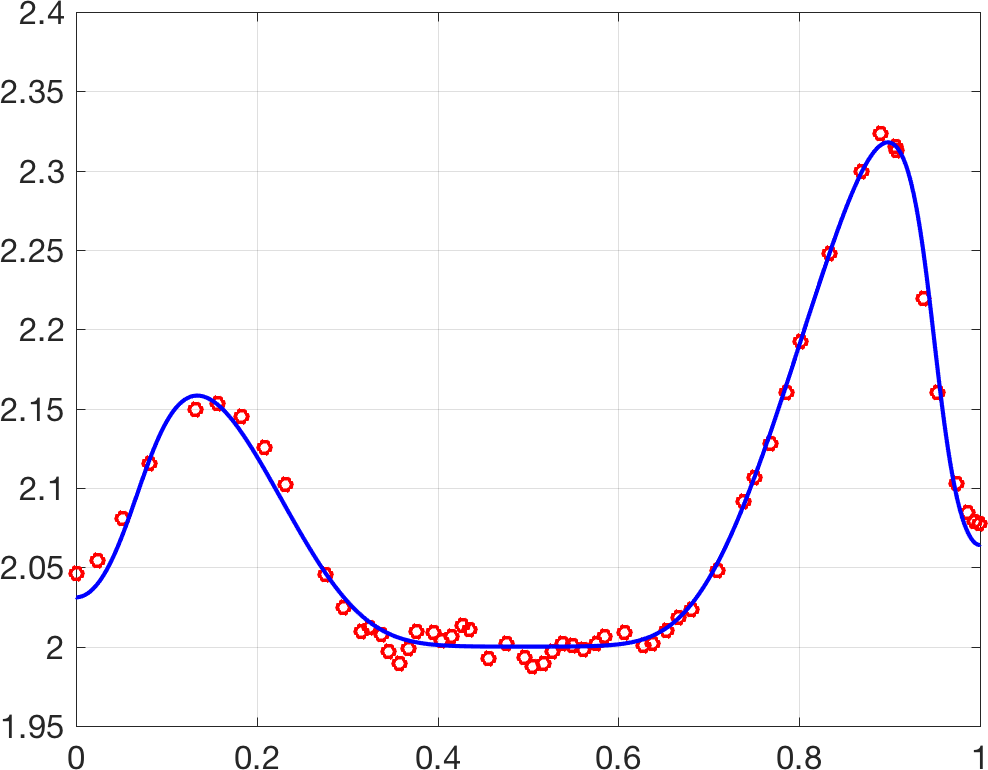
\includegraphics[width=.45\textwidth]{figs/euler1Dwall_t25_25modes.png}}
\hspace{.5em}
\subfloat[25 modes, 100 ECP, $T=.75$]{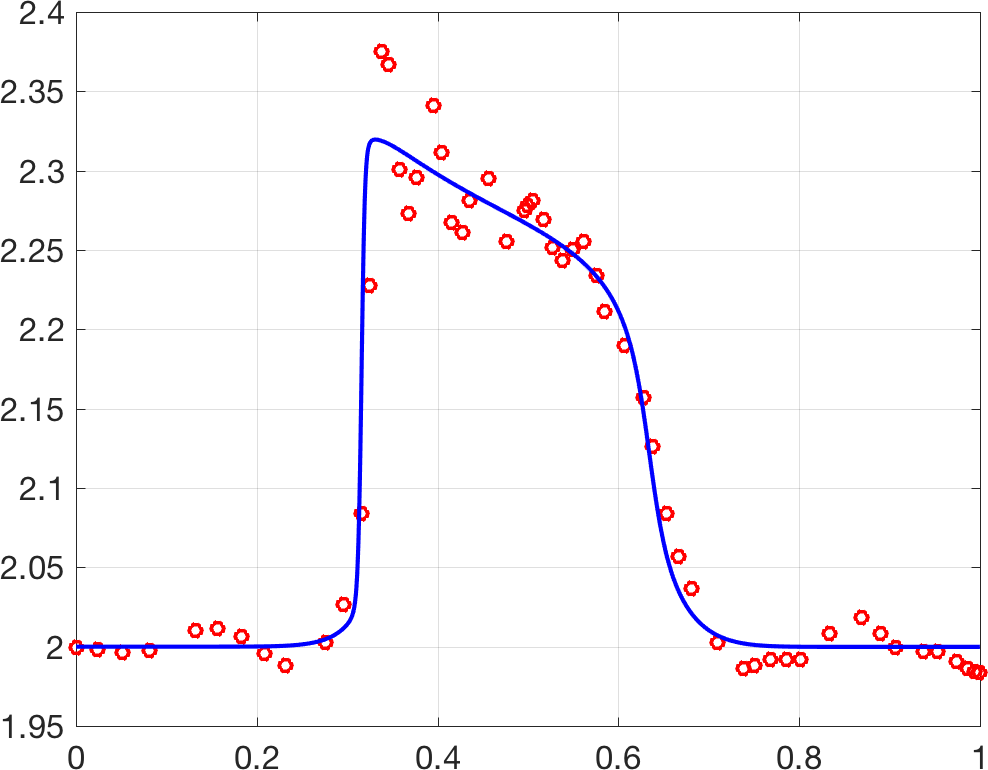
\includegraphics[width=.45\textwidth]{figs/euler1Dwall_t75_25modes.png}}
\caption*{\footnotesize FOM with $2500$ grid points, viscosity coefficient $\epsilon = 2e-4$, ROM with 25 modes.}
}
\only<2>{
\subfloat[75 modes, 205 ECP, $T=.25$]{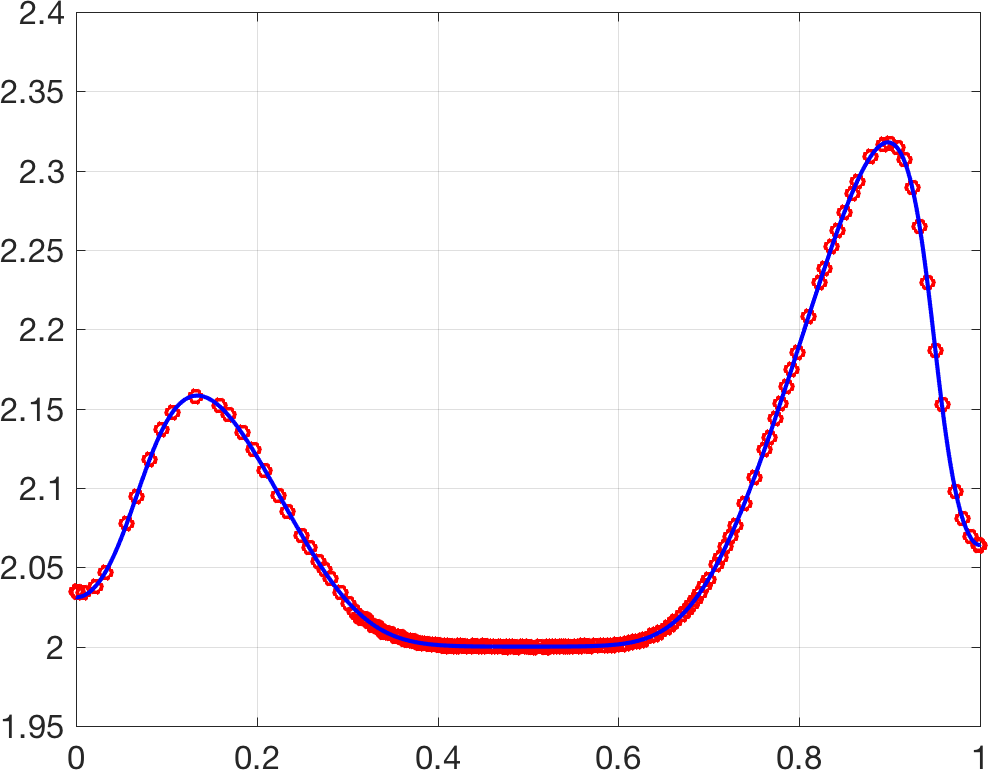
\includegraphics[width=.45\textwidth]{figs/euler1Dwall_t25_75modes.png}}
\hspace{.5em}
\subfloat[75 modes, 205 ECP, $T=.75$]{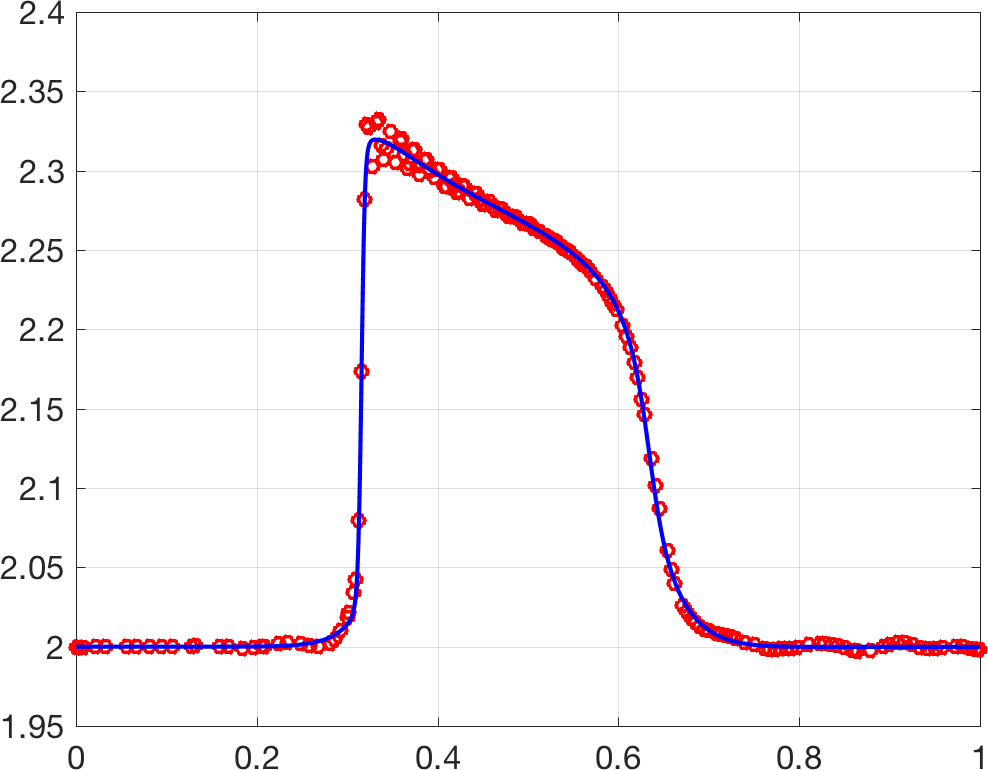
\includegraphics[width=.45\textwidth]{figs/euler1Dwall_t75_75modes.png}}
\caption*{\footnotesize FOM with $2500$ grid points, viscosity coefficient $\epsilon = 2e-4$, ROM with 75 modes.}
}
\only<3>{
\subfloat[125 modes, 304 ECP, $T=.25$]{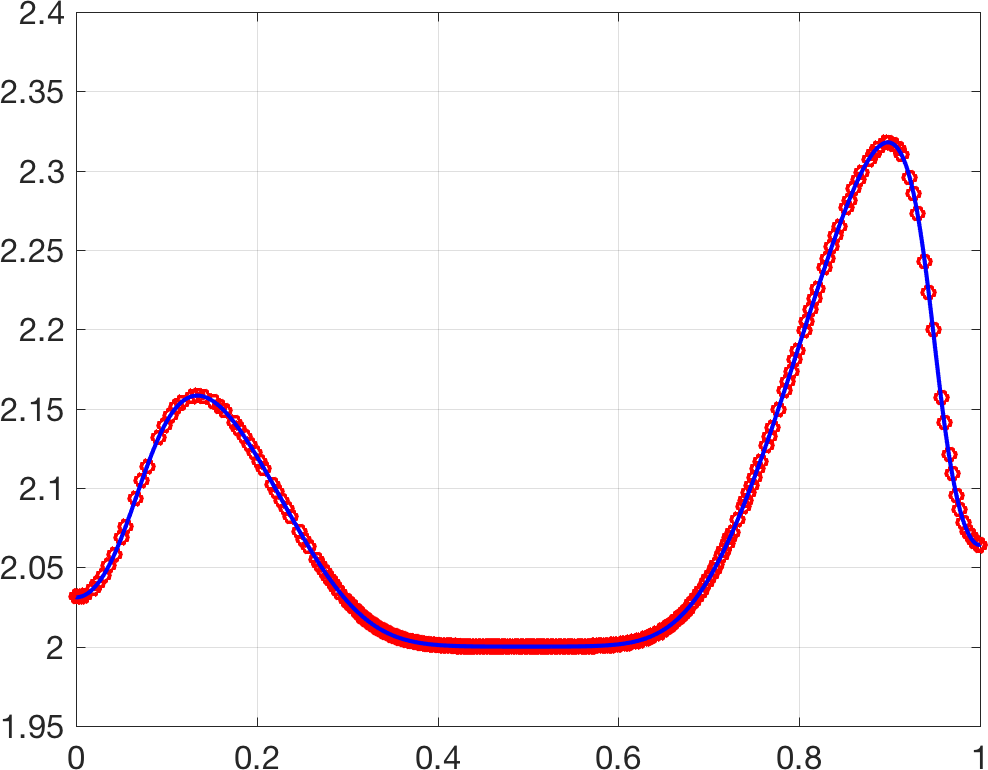
\includegraphics[width=.45\textwidth]{figs/euler1Dwall_t25_125modes.png}}
\hspace{.5em}
\subfloat[125 modes, 304 ECP, $T=.75$]{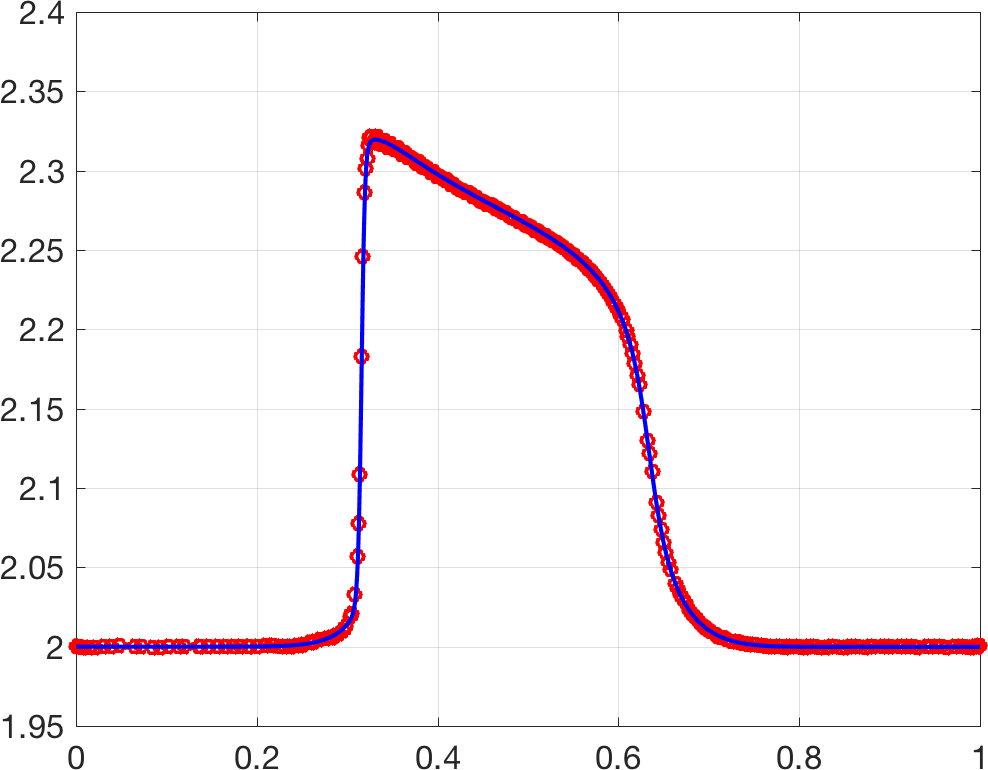
\includegraphics[width=.45\textwidth]{figs/euler1Dwall_t75_125modes.png}}
\caption*{\footnotesize FOM with $2500$ grid points, viscosity coefficient $\epsilon = 2e-4$, ROM with 125 modes.}
}
\end{figure}

\begin{center}
All results use explicit RK-45 time-stepping with FOM time-step.
\end{center}
}

\frame{
\frametitle{Evolution of average entropy}

\begin{figure}
\centering 
\only<1>{
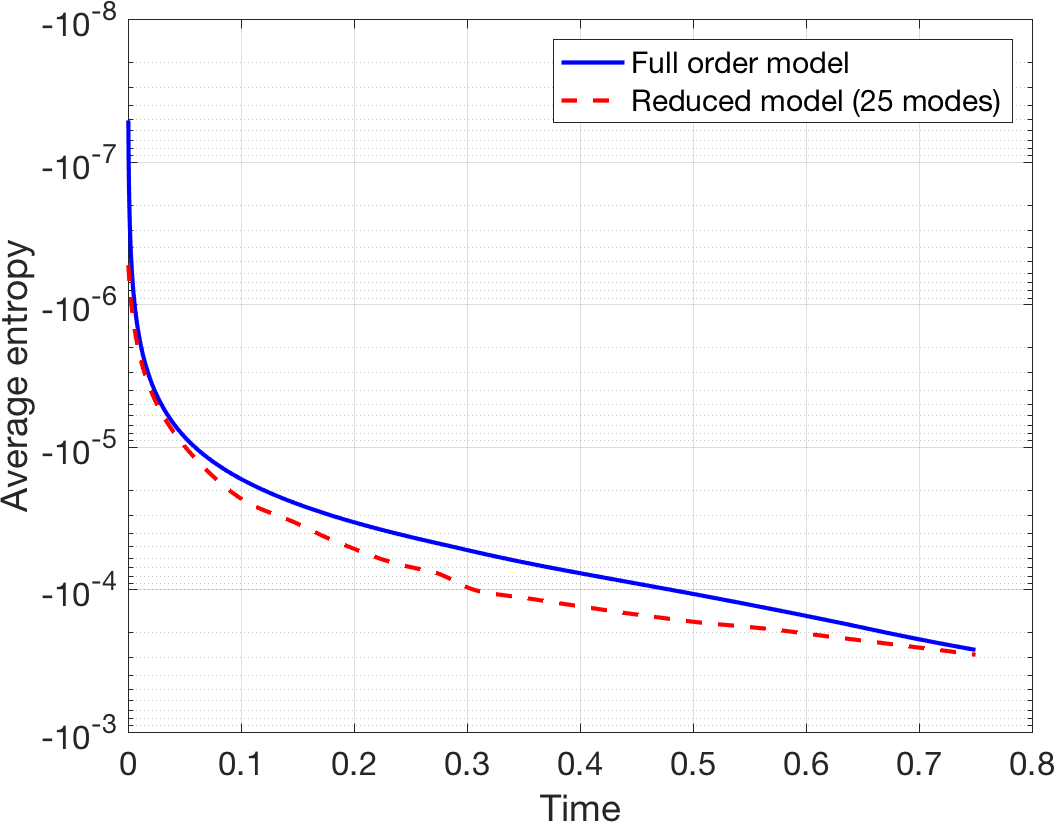
\includegraphics[width=.7\textwidth]{figs/euler1Dwall_entropy_25modes.png}
\caption*{Average entropy over time (25 modes).}
}
\only<2>{
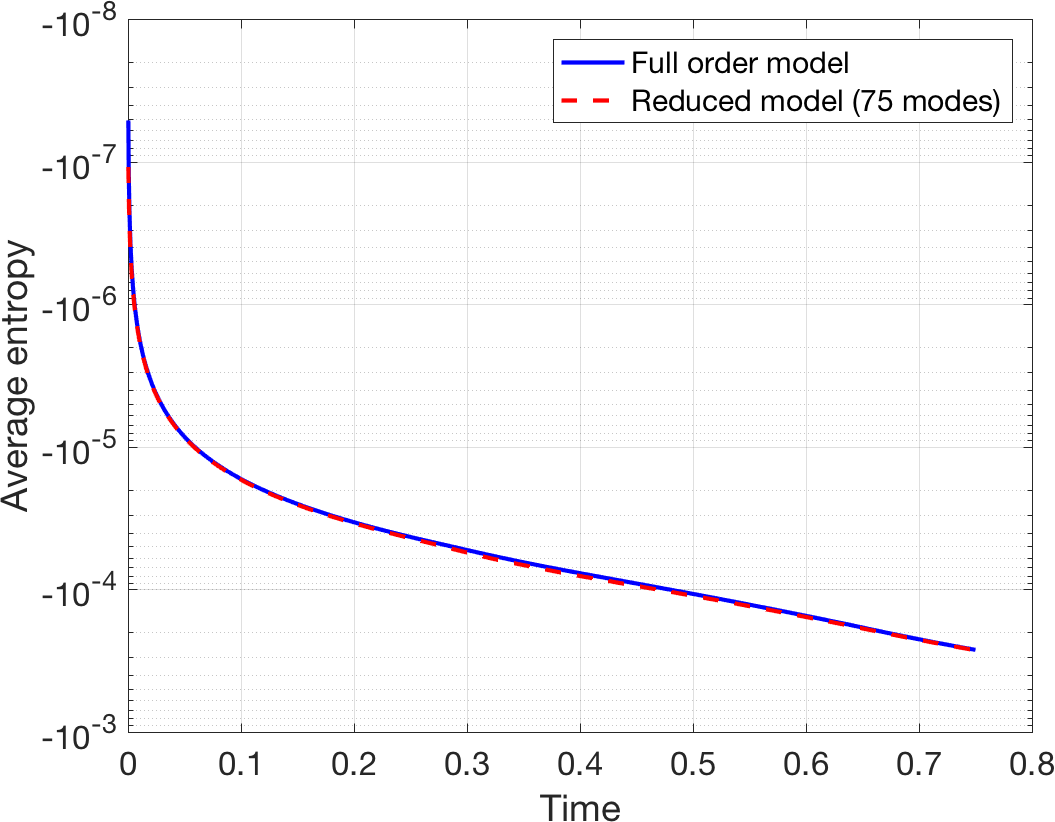
\includegraphics[width=.7\textwidth]{figs/euler1Dwall_entropy_75modes.png}
\caption*{Average entropy over time (75 modes).}
}
\only<3>{
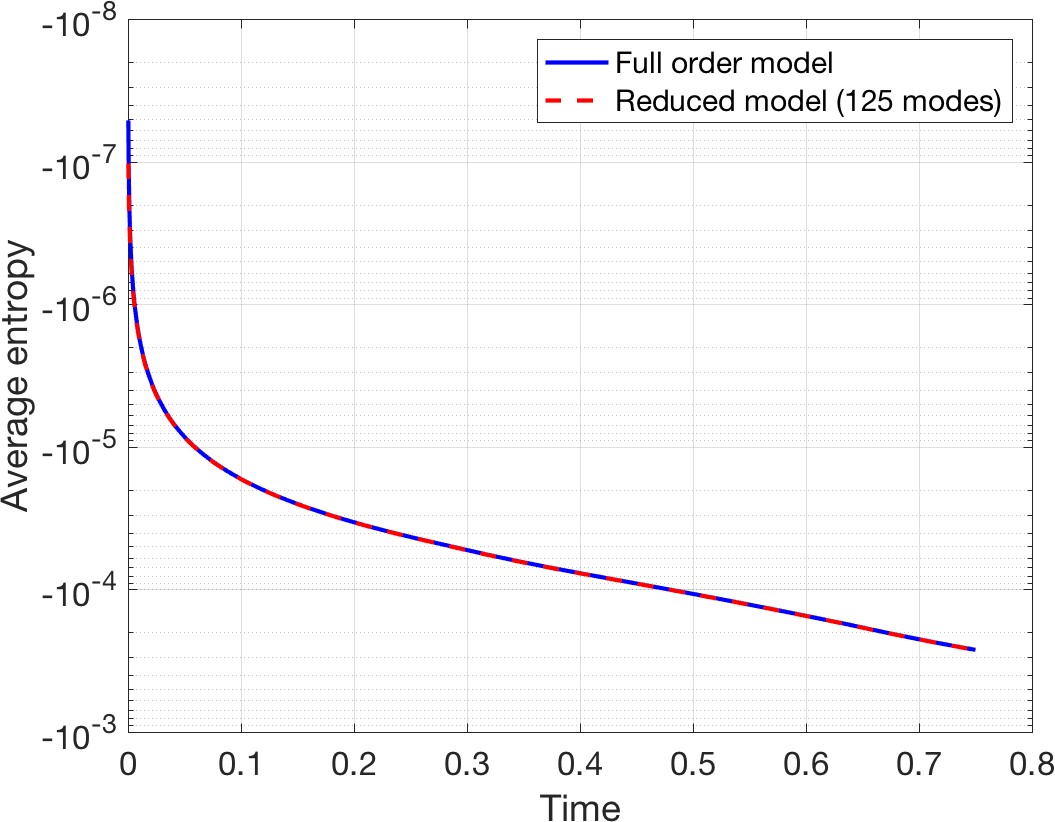
\includegraphics[width=.7\textwidth]{figs/euler1Dwall_entropy_125modes.png}
\caption*{Average entropy over time (125 modes).}
}
\end{figure}
}

\frame{
\frametitle{Error with and without hyper-reduction}
\vspace{-.5em}
\begin{figure}
\centering
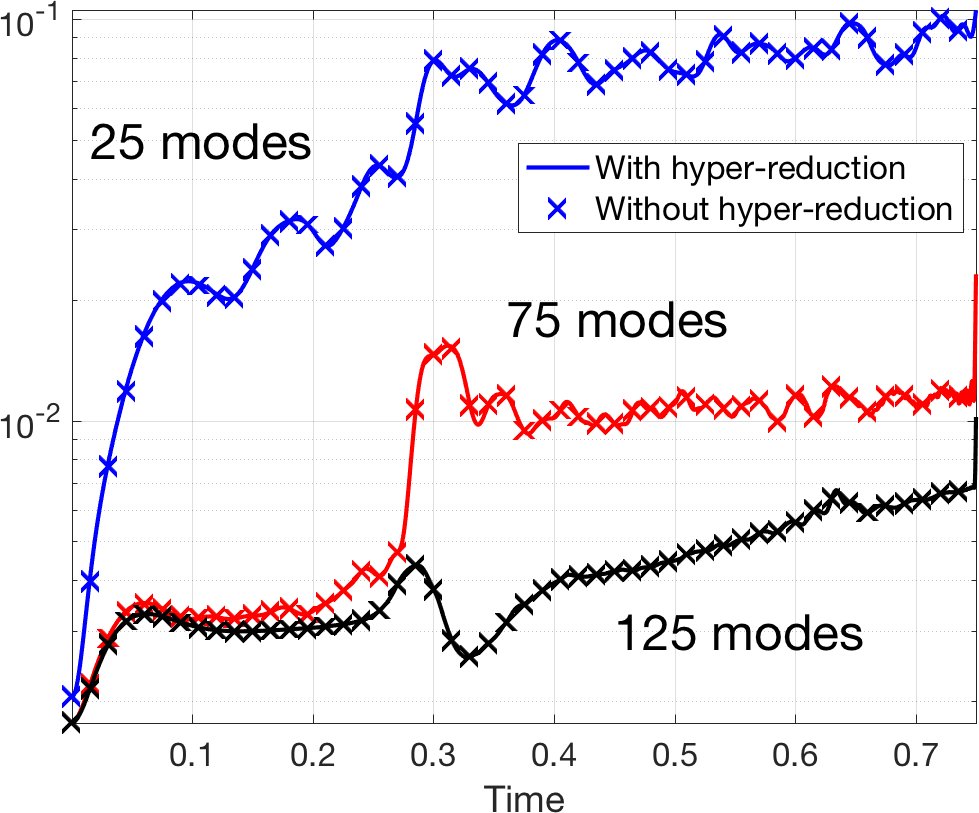
\includegraphics[width=.75\textwidth]{figs/euler_error_hypred_comparison_K2500.png}
\caption{Error over time for a $K=2500$ FOM and ROM with $25, 75, 125$ modes.}
\end{figure}
}

\frame{
\frametitle{Numerical results: smoothed Kelvin-Helmholtz instability}
\vspace{-.5em}
\begin{figure}
\centering 
\only<1>{
\subfloat[Density, full order model]{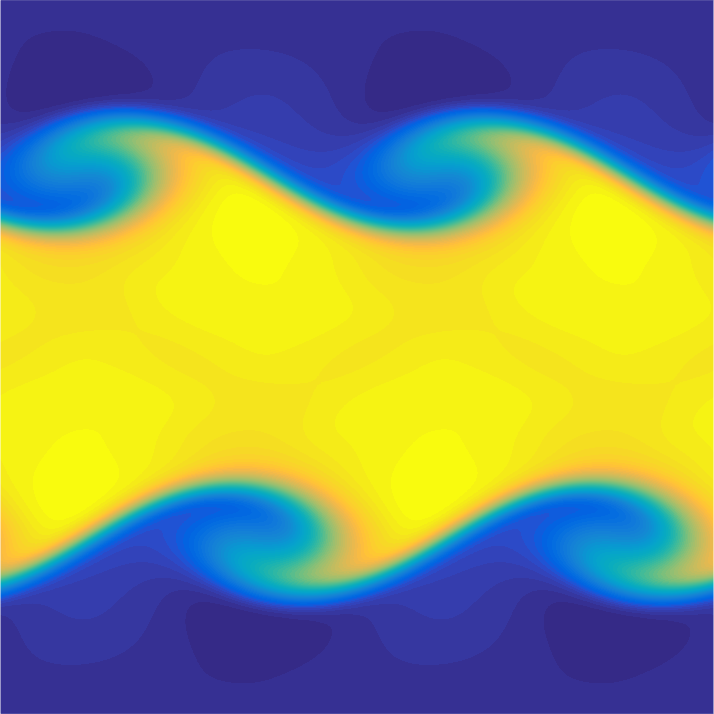
\includegraphics[width=.45\textwidth]{figs/khfom.png}}
\hspace{.5em}
\subfloat[Reduced order model]{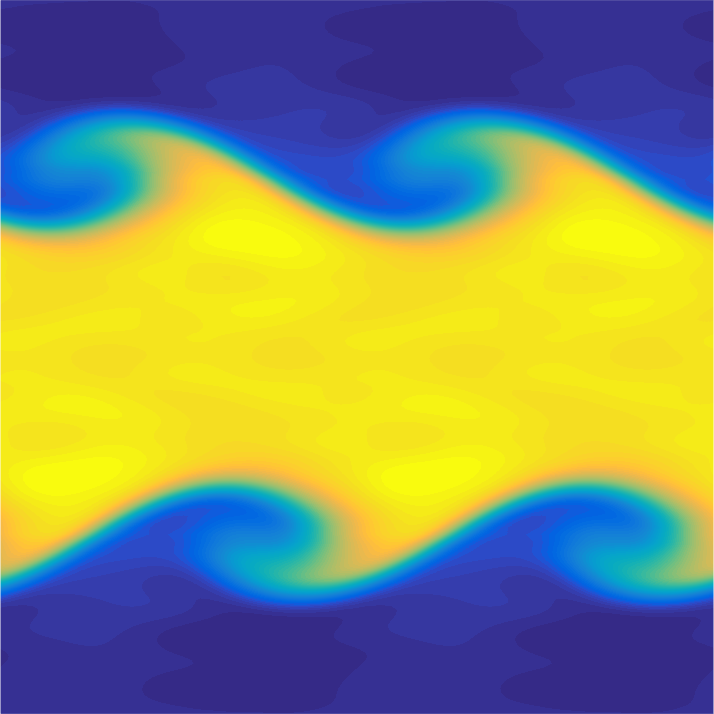
\includegraphics[width=.45\textwidth]{figs/khrom_75.png}}
}
\only<2>{
\subfloat[Density, full order model]{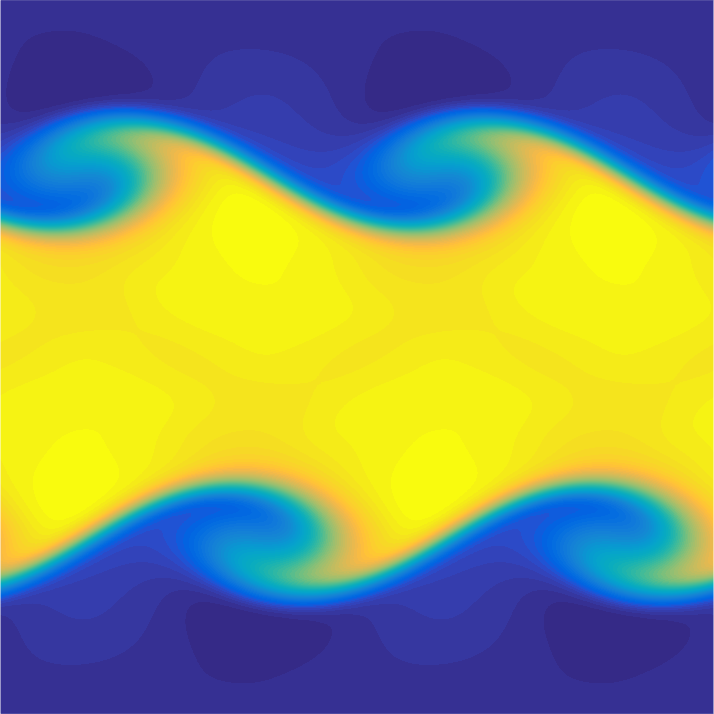
\includegraphics[width=.45\textwidth]{figs/khfom.png}}
\hspace{.5em}
\subfloat[ROM w/reduced quad.\ points]{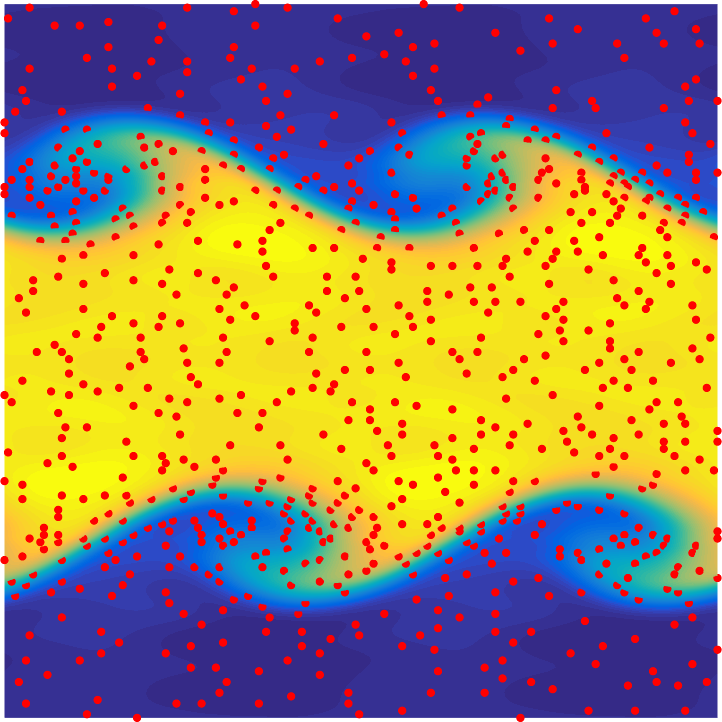
\includegraphics[width=.45\textwidth]{figs/khrom_75_ecp865.png}}
}
\caption{Full order model with $40000$ points, viscosity $\epsilon = .5\Delta x$.  ROM with $75$ modes, $865$ reduced quadrature points, $1.11 \%$ relative $L^2$ error at $T = 2.5$.}
\end{figure}
}

\frame{
\frametitle{Numerical results: Gaussian pulse with reflective wall}

\begin{figure}
\centering 
\only<1>{
\subfloat[Density, full order model]{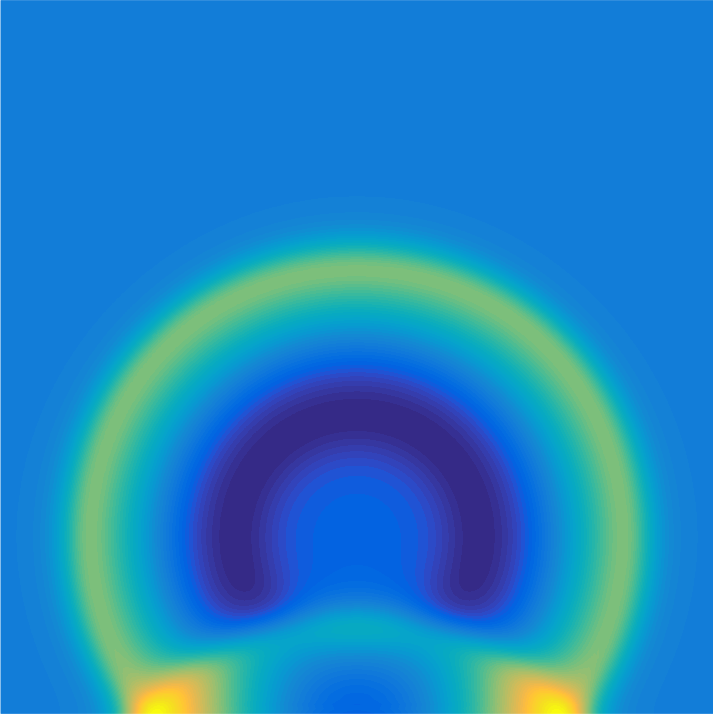
\includegraphics[width=.45\textwidth]{figs/pulse2d.png}}
\hspace{.5em}
\subfloat[Reduced order model]{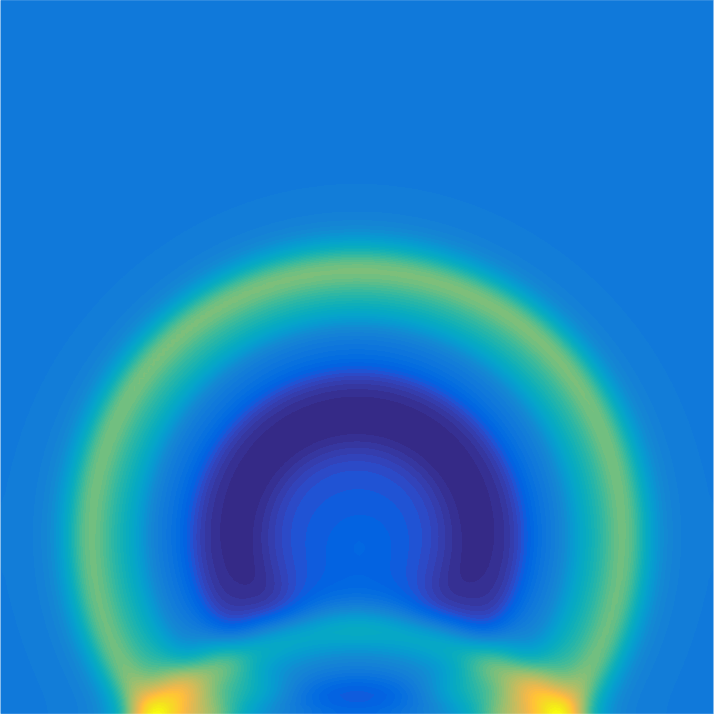
\includegraphics[width=.45\textwidth]{figs/pulse2d_ROM.png}}
}
\only<2>{
\subfloat[Density, full order model]{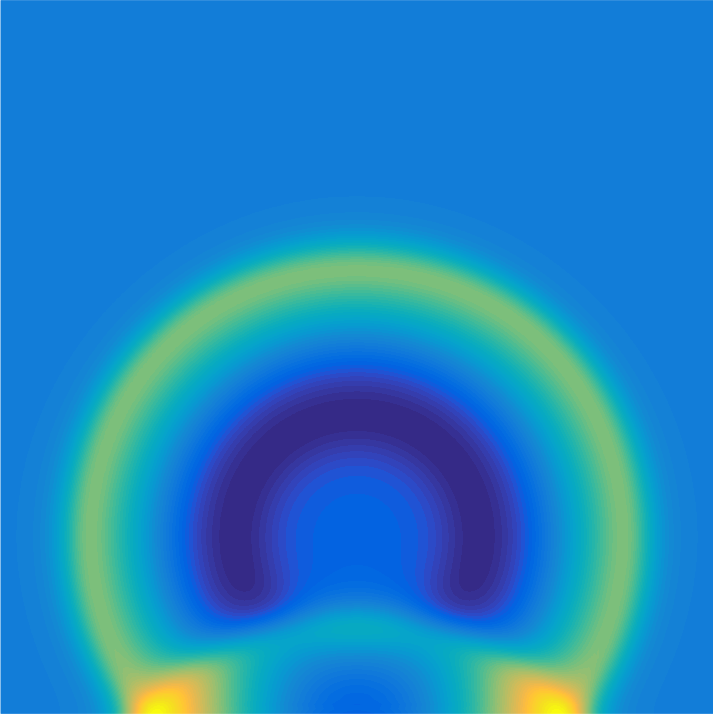
\includegraphics[width=.45\textwidth]{figs/pulse2d.png}}
\hspace{.5em}
\subfloat[ROM w/reduced quad.\ points]{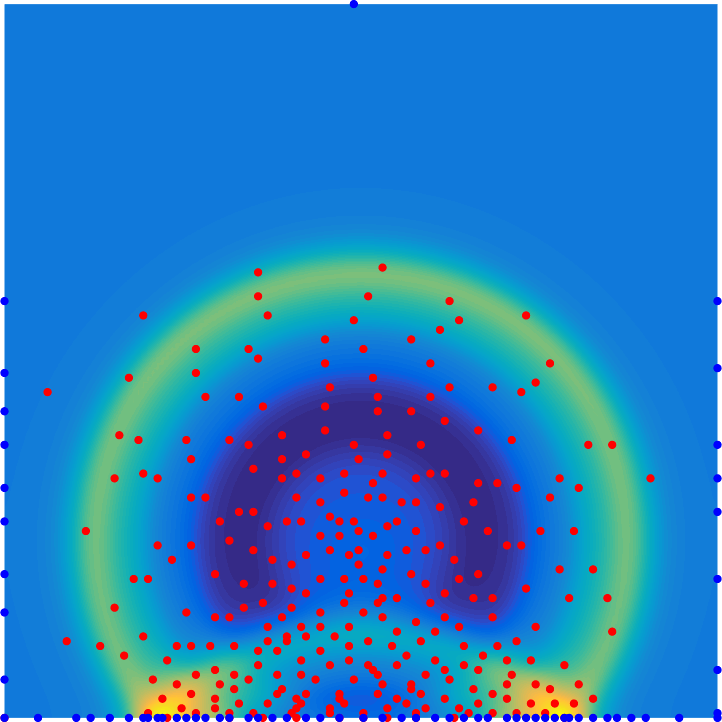
\includegraphics[width=.45\textwidth]{figs/pulse2d_ROM_pts.png}}
}
\caption{FOM with $10000$ points, viscosity $\epsilon = .5\Delta x$.  ROM with $25$ modes, $306$ reduced volume points, 82 reduced surface points, $.57 \%$ error at $T = .25$.}
\end{figure}

}
%% =================================================

\frame{
\frametitle{Summary and future work}

\begin{itemize}
\item Entropy stable reduced order models reproduces a semi-discrete evolution of entropy from the full order model.  
\item Open challenges: volume and surface hyper-reduction strategies, CFL and error analysis, approximation of convective solutions.
%\vspace{.25em}
%\item Current work: ROM, positivity preservation.  
\vspace{.25em}
%\item Current work: hybrid and non-conforming meshes, multi-GPU.
%\vspace{.25em}
\item This work is supported by DMS-1719818 and DMS-1712639. 
\end{itemize}
\vspace{.25em}
\begin{center}
Thank you!  Questions?
\vspace{.25em}

{
\includegraphics[width=.15\textwidth]{figs/nsf.jpg}}
\end{center}

\let\thefootnote\relax\footnotetext{\tiny Chan (In preparation). \textit{Entropy stable reduced order modeling of nonlinear conservation laws}.}
\let\thefootnote\relax\footnotetext{\tiny Chan (2019). \textit{Skew-symmetric entropy stable modal discontinuous Galerkin formulations}.}
\let\thefootnote\relax\footnotetext{\tiny Chan (2018). \textit{On discretely entropy conservative and entropy stable discontinuous Galerkin methods.}}
}

%% =================================================

\frame[noframenumbering]{
\frametitle{Additional slides}
}

\frame[noframenumbering]{
\frametitle{Example of entropy conservative finite volume fluxes}

\begin{itemize}
\item Entropy conservative flux for Burgers' equation 
\[
f_S(u_L,u_R) = \frac{1}{6}\LRp{u_L^2 + u_Lu_R + u_R^2}.
\]
\item Flux differencing: let $u_L = u(x), u_R = u(y)$
\begin{align*}
\pd{{f}({u})}{x} &\Longrightarrow \note{\LRu{2\pd{f_S\LRp{u(x),u(y)}}{x}}_{y=x}}
\end{align*}
\item Recovering the Burgers' split formulation
\begin{align*}
f_S(u(x),u(y)) &= \frac{1}{6}\LRp{u(x)^2 + u(x)u(y) + u(y)^2}\\
\LRu{2\pd{f_S\LRp{u(x),u(y)}}{x}}_{y=x} &= \frac{1}{3}\pd{u^2}{x} + \frac{1}{3}u\pd{u}{x} + \frac{1}{3}u^2\cancel{\pd{1}{x}}.
\end{align*}
\end{itemize}
}


\frame[noframenumbering]{
\frametitle{Entropy conservative fluxes for compressible Euler}
\begin{itemize}
\item In one dimension:
\begin{align*}
f^1_S(\bm{u}_L,\bm{u}_R) &= \avg{\rho}^{\log} \avg{u}\\
f^2_S(\bm{u}_L,\bm{u}_R) &= \frac{\avg{\rho}}{2\avg{\beta}} + \avg{u}f^1_S\\
f^3_S(\bm{u}_L,\bm{u}_R) &= f^1_S\LRp{\frac{1}{2(\gamma-1)\avg{\beta}^{\log}} - \frac{1}{2}\avg{u^2}} + \avg{u}f^2_S,
\end{align*}
\vspace{.5em}
\item Involves logarithmic mean and ``inverse temperature'' $\beta$
\[
\avg{u}^{\log} = \frac{u_L - u_R}{\log{u_L}- \log{u_R}}, \qquad \beta = \frac{\rho}{2p}.
\]
\end{itemize}

\let\thefootnote\relax\footnotetext{\tiny Chandreshekar (2013),  \emph{Kinetic energy preserving and entropy stable FV schemes for comp.\ Euler and NS equations.}}
}

\frame[noframenumbering]{
\frametitle{Determining empirical cubature points (ECP) and weights}

\begin{itemize}
\item Goal: integrate a target basis to some accuracy.
\vspace{1em}
\item Offline step: greedy selection of hyper-reduction points
\begin{itemize}
\item Project residual onto remaining rows of basis matrix.
\item Find ``most positive'' point of projected residual.
\item Solve (nonlinear) least squares for (positive) quadrature weights.
\end{itemize}
\vspace{1em}
\item Target basis: products of modes
\[
{\rm span}\LRc{\phi_i(\bm{x})\phi_j(\bm{x}), \quad 1\leq i,j \leq N}.
\]
Reduce costs by substituting leading POD modes.  
%\vspace{1em}
%\item Number of EC points depends on FOM viscosity, smoothness.  
\end{itemize}

\let\thefootnote\relax\footnotetext{\tiny Hernandez, Caicedo, Ferrer (2017).  \textit{Dimensional hyper-reduction of nonlinear finite element models via empirical cubature.}}
}



\end{document}
